%% Cloud Databases: A Systematic Meta-Survey
%% For Data & Knowledge Engineering (Elsevier)
%% Elsevier CAS single-column document class (cas-sc), numbered citations
%%
\documentclass[a4paper,fleqn]{cas-sc}

%% natbib in numbered mode -> [1]-style citations
\usepackage[numbers]{natbib}

%% Packages NOT already provided by cas-sc.
%% (cas-sc already loads: graphicx, amsmath/amsfonts/amssymb, booktabs,
%%  makecell, multirow, array, colortbl, xcolor, hyperref.)
\usepackage{tabularx}
\usepackage{longtable}
\usepackage{rotating}
\usepackage{pdflscape}
\usepackage{tikz}
\usepackage{pgfplots}
\pgfplotsset{compat=1.18}
\usetikzlibrary{shapes.geometric, arrows.meta, positioning, calc, patterns, fit, backgrounds, decorations.markings}
\usepackage{enumitem}
\usepackage{float}
\restylefloat{figure} %% enable the [H] (exact placement) specifier for the CAS figure float
\usepackage{adjustbox}

%% Symbols for challenge coverage matrix
\newcommand{\FULL}{\raisebox{-0.3ex}{$\bullet$}}
\newcommand{\PART}{$\circ$}
\newcommand{\MINOR}{$\cdot$}
\newcommand{\rot}[1]{\rotatebox{90}{\parbox{2.2cm}{\raggedright\small #1}}}

%% Color definitions for figures
%% Grayscale palette: all figures are rendered in black and white.
%% The original color names are retained but remapped to gray levels, so
%% every figure (which references these macros) becomes monochrome at once.
\definecolor{cblue}{gray}{0.45}
\definecolor{corange}{gray}{0.62}
\definecolor{cgray}{gray}{0.72}
\definecolor{cyellow}{gray}{0.82}
\definecolor{clblue}{gray}{0.55}
\definecolor{cgreen}{gray}{0.70}
\definecolor{cdblue}{gray}{0.25}
\definecolor{cred}{gray}{0.38}
\definecolor{cpurple}{gray}{0.50}
\definecolor{cteal}{gray}{0.60}

\begin{document}
\let\WriteBookmarks\relax

\shorttitle{Cloud Databases: A Systematic Meta-Survey}
\shortauthors{A. Ibrahim}

\title[mode=title]{Cloud Databases: A Systematic Meta-Survey of Current Challenges, Emerging Paradigms, and Future Research Directions}

\author[1]{Abdulhakeem Ibrahim}[orcid=0000-0002-1104-5314]
\cormark[1]
\ead{hakeem.ibrahim@dmu.ac.uk}

\affiliation[1]{organization={School of Computer Science and Informatics, De Montfort University},
            city={Leicester},
            country={United Kingdom}}

\cortext[1]{Corresponding author.}

\begin{abstract}
Cloud databases have become the backbone of modern data-driven applications, enabling organizations to store, process, and analyze data at unprecedented scale and elasticity. Over more than two decades (1999--2026), 96 survey papers satisfying systematic inclusion and quality criteria have examined various facets of cloud database technology---spanning cloud-native architectures, hybrid transactional and/or analytical processing (HTAP), NoSQL/NewSQL systems, vector and graph databases, AI-for-database optimization (AI4DB), data lakehouses, time-series databases, cloud database migration, and edge--cloud data management. However, the challenges, open problems, and research directions identified in these surveys remain fragmented across disparate communities and publication venues. This paper presents the first \emph{systematic meta-survey} of cloud database research: a survey of surveys that synthesizes findings from carefully selected survey papers using a rigorous methodology grounded in the Kitchenham--Charters systematic literature review protocol. The scattered landscape of cloud database challenges is organized into a structured, dual-theme taxonomy: (1)~\emph{eighteen cross-cutting challenges} that transcend individual system categories, including scalability, consistency trade-offs, security, cost optimization, AI--database convergence, and sustainability; and (2)~\emph{five lifecycle-phase challenges} spanning design, deployment, operation, optimization, and evolution of cloud database systems. The convergence of cloud databases with large language models (LLMs) is further examined as an illustrative case study, and a consolidated set of open research directions is distilled from the cross-survey synthesis. By providing a consolidated, thematically organized view of the field, this meta-survey serves as both a comprehensive reference for researchers entering the cloud database space and a strategic guide for practitioners navigating the rapidly evolving landscape of cloud data management.
\end{abstract}

%% Highlights are submitted to Elsevier as a separate file (not a manuscript page).
%% Kept here for reference:
%% - First systematic meta-survey of 96 cloud database surveys (1999--2026 search window)
%% - Dual-theme taxonomy: 18 cross-cutting and 5 lifecycle-phase challenges
%% - Cross-survey synthesis of consensus and divergence on each challenge
%% - Cloud database and large language model convergence as a case study
%% - Consolidated cross-cutting research agenda distilled from the synthesis

\begin{keywords}
cloud databases \sep systematic meta-survey \sep cloud-native databases \sep database-as-a-service \sep data lakehouse \sep AI4DB \sep survey of surveys
\end{keywords}

\maketitle

%% ============================================================
%% SECTION 1: INTRODUCTION
%% ============================================================
\section{Introduction}
\label{sec:introduction}

The cloud database market has experienced explosive growth over the past decade, with global revenues projected to exceed \$200 billion by 2028~\cite{gartner2024dbms}. This growth reflects a fundamental shift in how organizations manage data: from on-premises, monolithic database servers to elastic, globally distributed, cloud-native data platforms that can scale storage and compute independently on demand~\cite{Verbitski2017,Dageville2016}. Major cloud providers---Amazon Web Services (AWS), Microsoft Azure, Google Cloud Platform (GCP), and Alibaba Cloud---now offer dozens of specialized database services, from relational engines like Amazon Aurora~\cite{Verbitski2017} and Azure SQL~\cite{Antonopoulos2019} to purpose-built systems for documents, graphs, time series, key-value pairs, and, most recently, vector embeddings for AI workloads~\cite{Pan2024VectorDB}.

This rapid evolution has attracted significant research attention. A scripted search across four scholarly indexing services (OpenAlex, arXiv, Crossref, and Semantic Scholar) covering January 1999 to July 2026 identifies \textbf{96 survey papers} meeting the inclusion and quality criteria, each examining a particular facet of cloud database technology. These surveys span a wide spectrum of topics: cloud-native database architectures~\cite{Li2024CloudNativeSurvey}, hybrid transactional/analytical processing (HTAP)~\cite{Haas2024HTAPSurvey}, graph databases~\cite{Angles2020GraphDB}, vector database management systems~\cite{Pan2024VectorDB}, AI-driven database optimization (AI4DB)~\cite{Zhou2022AI4DB}, data lakehouses~\cite{Harby2022Lakehouse}, NoSQL and NewSQL systems~\cite{Davoudian2018NoSQL,Kaur2021NoSQLReview}, edge and fog database systems~\cite{Gomes2024EdgeFog}, and many more.

Despite this wealth of individual surveys, the field lacks a \emph{meta-level synthesis}---a comprehensive, systematic effort to consolidate the challenges, open problems, and research directions scattered across these surveys into a unified framework. Each survey naturally focuses on its own domain, leading to a fragmented understanding of the cloud database landscape as a whole. Cross-cutting challenges such as cost optimization, security, consistency trade-offs, and AI--database convergence are discussed in many surveys but from different angles, without a common organizing framework.

\subsection{Contributions and novelty}
\label{subsec:contributions}

This paper addresses the gap by presenting the \textbf{first systematic meta-survey of cloud database research}---a survey of surveys. A rigorous systematic literature review (SLR) protocol based on the Kitchenham--Charters guidelines~\cite{Kitchenham2007} is applied to identify, evaluate, and synthesize cloud database surveys. The contributions of this work are as follows:

\begin{enumerate}[label=\textbf{C\arabic*}]
    \item \textbf{Systematic identification and classification.} Four scholarly APIs are searched with a fully scripted, reproducible protocol over the window January 1999 to July 2026, yielding 96 quality-assessed survey papers on cloud databases, classified by topic, scope, methodology, and venue.

    \item \textbf{Dual-theme challenge taxonomy.} The scattered challenges are organized into a structured taxonomy with two complementary themes:
    \begin{itemize}
        \item \emph{Theme~1: Eighteen cross-cutting challenges} that recur across multiple survey domains, including scalability, consistency, security, cost modeling, AI--database convergence, and sustainability.
        \item \emph{Theme~2: Five lifecycle-phase challenges} that map to the stages of designing, deploying, operating, optimizing, and evolving cloud database systems.
    \end{itemize}

    \item \textbf{LLM--database convergence analysis.} The rapidly emerging intersection of large language models (LLMs) and cloud databases is examined as an illustrative case study, covering text-to-SQL, vector databases for retrieval-augmented generation (RAG), and LLM-based database administration.

    \item \textbf{Research agenda.} A consolidated, cross-cutting research agenda is distilled from the synthesis, grouping the open problems that recur most widely across the surveyed literature.

    \item \textbf{Knowledge engineering perspective.} Cloud database challenges are explicitly connected to data and knowledge engineering concerns---including knowledge graphs, ontologies, metadata management, and schema evolution---making this survey particularly relevant to the \emph{Data \& Knowledge Engineering} community.
\end{enumerate}

\subsection{Research questions}
\label{subsec:rqs}

This meta-survey is guided by five research questions, summarized in Table~\ref{tab:rqs} and elaborated in Section~\ref{sec:methodology}.

\begin{table}[H]
\centering
\caption{Research questions guiding the meta-survey.}
\label{tab:rqs}
\small
\begin{tabular}{c p{10cm}}
\toprule
\textbf{ID} & \textbf{Research Question} \\
\midrule
RQ1 & What is the landscape of cloud database surveys published between 1999 and 2026, in terms of topic coverage, methodology, and publication venue? \\
\addlinespace
RQ2 & What are the major cross-cutting challenges identified across cloud database surveys, and how do they relate to one another? \\
\addlinespace
RQ3 & How do cloud database challenges map to the lifecycle phases of designing, deploying, operating, optimizing, and evolving database systems? \\
\addlinespace
RQ4 & What is the current state and future trajectory of the convergence between cloud databases and AI/ML technologies, particularly large language models? \\
\addlinespace
RQ5 & What are the most pressing open research directions, and which of them recur most widely across the surveyed literature? \\
\bottomrule
\end{tabular}
\end{table}

\subsection{Paper organization}
\label{subsec:organization}

The remainder of this paper is organized as shown in Figure~\ref{fig:organization}. Section~\ref{sec:motivation} motivates the importance of cloud databases from five complementary perspectives. Section~\ref{sec:concepts} establishes key definitions and distinctions---from cloud-hosted to cloud-native databases, architectural paradigms, data models, and the data platform continuum. Section~\ref{sec:methodology} details the systematic review methodology, including search strategy, selection criteria, quality assessment, and results. Section~\ref{sec:discussion} presents the core contribution: a comprehensive discussion of challenges and research directions organized by cross-cutting themes and lifecycle phases. Section~\ref{sec:llm} examines the convergence of cloud databases and LLMs. Section~\ref{sec:conclusion} concludes. Appendix~\ref{app:catalog} provides the complete catalog of surveyed papers.

\begin{figure}[H]
\centering
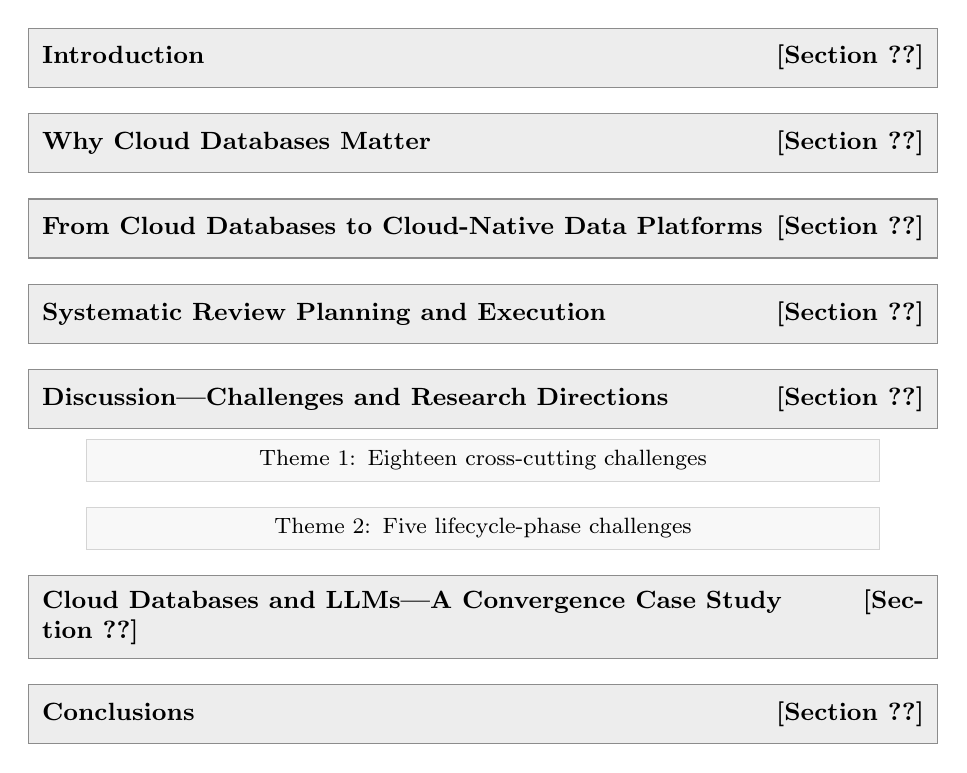
\begin{tikzpicture}[
    node distance=0.32cm,
    secbox/.style={draw, fill=cgray!25, draw=cdblue!60, text width=11.2cm, minimum height=0.75cm, align=left, font=\small\bfseries, inner sep=5pt},
    subbox/.style={draw, fill=cgray!10, draw=cgray!60, text width=9.8cm, minimum height=0.5cm, align=center, font=\footnotesize, inner sep=4pt}
]
\node[secbox] (s1) {Introduction \hfill [Section~\ref{sec:introduction}]};
\node[secbox, below=of s1] (s2) {Why Cloud Databases Matter \hfill [Section~\ref{sec:motivation}]};
\node[secbox, below=of s2] (s3) {From Cloud Databases to Cloud-Native Data Platforms \hfill [Section~\ref{sec:concepts}]};
\node[secbox, below=of s3] (s4) {Systematic Review Planning and Execution \hfill [Section~\ref{sec:methodology}]};
\node[secbox, below=of s4] (s5) {Discussion---Challenges and Research Directions \hfill [Section~\ref{sec:discussion}]};
\node[subbox, below=0.12cm of s5] (s5a) {Theme 1: Eighteen cross-cutting challenges};
\node[subbox, below=of s5a] (s5b) {Theme 2: Five lifecycle-phase challenges};
\node[secbox, below=0.32cm of s5b] (s6) {Cloud Databases and LLMs---A Convergence Case Study \hfill [Section~\ref{sec:llm}]};
\node[secbox, below=of s6] (s7) {Conclusions \hfill [Section~\ref{sec:conclusion}]};
\end{tikzpicture}
\caption{The organization of this meta-survey paper.}
\label{fig:organization}
\end{figure}


%% ============================================================
%% SECTION 2: MOTIVATION
%% ============================================================
\section{Why Cloud Databases Matter---A Multi-Perspective Motivation}
\label{sec:motivation}

Understanding the significance of cloud databases requires examining the topic from multiple viewpoints. In this section, the need for a meta-survey is motivated by discussing five complementary perspectives (Figure~\ref{fig:perspectives}), each revealing why the scattered state of survey knowledge is problematic and why a unified synthesis is timely.

\begin{figure}[H]
\centering
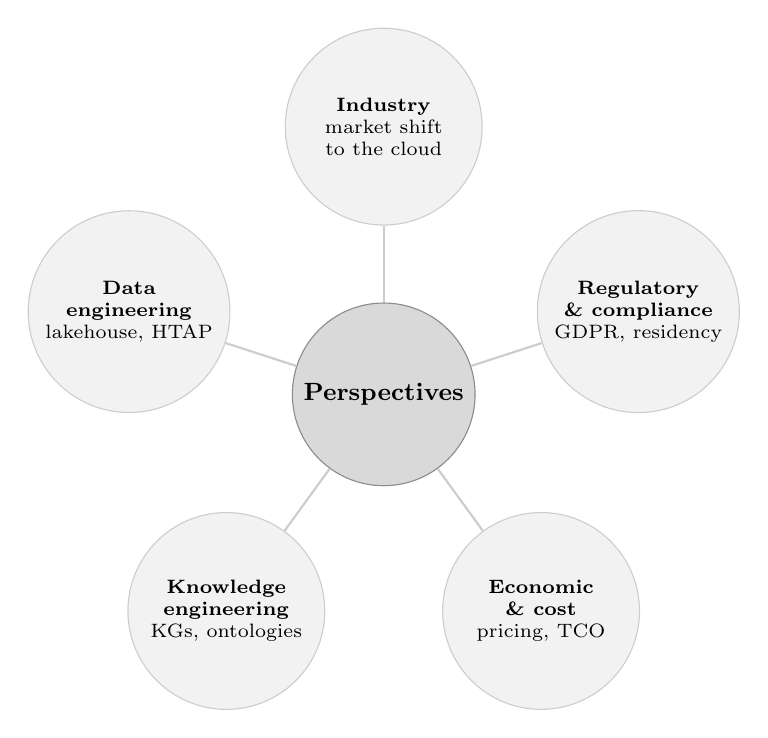
\begin{tikzpicture}[
    hub/.style={draw, circle, fill=cdblue!20, draw=cdblue!60, minimum size=2.0cm, align=center, font=\small\bfseries},
    persp/.style={draw, circle, fill=cgray!18, draw=cgray!70, minimum size=2.5cm, align=center, font=\scriptsize},
    spoke/.style={-, thick, cgray!70}
]
\node[hub] (h) at (0,0) {Perspectives};
\node[persp] (p1) at (90:3.4cm) {\textbf{Industry}\\market shift\\to the cloud};
\node[persp] (p2) at (162:3.4cm) {\textbf{Data}\\\textbf{engineering}\\lakehouse, HTAP};
\node[persp] (p3) at (234:3.4cm) {\textbf{Knowledge}\\\textbf{engineering}\\KGs, ontologies};
\node[persp] (p4) at (306:3.4cm) {\textbf{Economic}\\\textbf{\& cost}\\pricing, TCO};
\node[persp] (p5) at (18:3.4cm) {\textbf{Regulatory}\\\textbf{\& compliance}\\GDPR, residency};
\draw[spoke] (h) -- (p1);
\draw[spoke] (h) -- (p2);
\draw[spoke] (h) -- (p3);
\draw[spoke] (h) -- (p4);
\draw[spoke] (h) -- (p5);
\end{tikzpicture}
\caption{The five complementary perspectives motivating a systematic meta-survey of cloud databases.}
\label{fig:perspectives}
\end{figure}

\subsection{Industry perspective}
\label{subsec:industry}

The global database management system (DBMS) market reached \$101 billion in 2023, with cloud deployments accounting for over 65\% of total revenue---up from approximately 40\% in 2019~\cite{gartner2024dbms}. Gartner projects that by 2026, 75\% of all databases will be deployed on cloud platforms~\cite{gartner2024dbms}. This shift is driven by digital transformation initiatives across industries, from financial services adopting cloud databases for real-time fraud detection to healthcare organizations leveraging cloud data platforms for genomics and precision medicine~\cite{AmazonAurora2023}.

The vendor landscape has also diversified significantly. Beyond the hyperscale cloud providers (AWS, Azure, GCP), specialized cloud database vendors such as Snowflake~\cite{Dageville2016}, Databricks~\cite{Armbrust2021Lakehouse}, CockroachDB~\cite{Taft2020Cockroach}, PlanetScale, and Neon have gained substantial market share. China's cloud database ecosystem---including Alibaba PolarDB~\cite{Cao2021PolarDB}, TiDB~\cite{Huang2020TiDB}, and OceanBase~\cite{Yang2022OceanBase}---has matured rapidly. This fragmentation makes it difficult for practitioners to navigate the landscape without a systematic overview.

\subsection{Data engineering perspective}
\label{subsec:dataeng}

Modern data architectures have evolved from simple transactional databases to complex, multi-layered data ecosystems. The emergence of the \emph{data lakehouse} paradigm~\cite{Armbrust2021Lakehouse} exemplifies this evolution, combining the flexibility of data lakes with the governance and performance of data warehouses. Systems like Databricks Delta Lake, Apache Iceberg, and Apache Hudi have created a new ``open table format'' layer that bridges batch and streaming analytics~\cite{Harby2022Lakehouse}.

Simultaneously, the rise of \emph{HTAP} (Hybrid Transactional/Analytical Processing) systems~\cite{Haas2024HTAPSurvey} challenges the traditional separation between OLTP and OLAP workloads. Systems such as TiDB~\cite{Huang2020TiDB}, SAP HANA~\cite{Farber2012}, and Google AlloyDB promise unified engines that handle both transaction processing and analytical queries. Understanding the trade-offs, maturity, and open challenges of these paradigms requires synthesizing insights across multiple survey papers.

\subsection{Knowledge engineering perspective}
\label{subsec:ke}

Cloud databases play a crucial role in knowledge engineering, making this topic directly relevant to the \emph{Data \& Knowledge Engineering} (DKE) community. Several connections are worth highlighting:

\begin{itemize}
    \item \textbf{Knowledge graphs in the cloud.} Large-scale knowledge graphs (KGs) such as Google Knowledge Graph, Wikidata, and enterprise KGs are increasingly stored and queried using cloud-hosted graph databases (e.g., Amazon Neptune, Azure Cosmos DB with Gremlin API, Neo4j Aura)~\cite{Angles2020GraphDB,Elbattah2015Freebase,Coimbra2025GraphDB}. The scalability, consistency, and query optimization challenges of cloud graph databases directly impact KG applications.

    \item \textbf{Ontology-mediated data access.} Cloud environments with heterogeneous data sources benefit from ontology-based data integration (OBDI) techniques~\cite{Xiao2018OBDA}, where ontologies provide a unified conceptual layer over distributed cloud databases.

    \item \textbf{Metadata and schema management.} Cloud data catalogs and metadata management systems (e.g., AWS Glue Data Catalog, Apache Atlas) implement knowledge engineering principles for organizing, discovering, and governing data assets~\cite{Halevy2016Goods}.

    \item \textbf{AI--knowledge engineering convergence.} The integration of machine learning with database systems (AI4DB)~\cite{Zhou2022AI4DB} draws on knowledge engineering concepts such as learned models for query optimization, workload characterization, and automated tuning.
\end{itemize}

\subsection{Economic and cost perspective}
\label{subsec:cost}

Cloud databases introduce novel economic dynamics compared to on-premises deployments. The shift from capital expenditure (CapEx) to operational expenditure (OpEx) models, combined with pay-per-use pricing and complex multi-dimensional billing (compute, storage, I/O, network egress, backups), creates significant challenges in cost prediction and optimization~\cite{Leis2023CloudPricing,Mateljan2010ROI}.

Research has shown that cloud database costs can vary by orders of magnitude depending on configuration choices, query patterns, and pricing model selection~\cite{Leis2023CloudPricing}. The total cost of ownership (TCO) analysis becomes particularly complex for multi-cloud or hybrid cloud deployments. Several surveys touch on cost-related challenges~\cite{Li2024CloudNativeSurvey,Muller2020Serverless}, but a consolidated analysis is lacking.

\subsection{Regulatory and compliance perspective}
\label{subsec:regulatory}

Data sovereignty regulations such as the European Union's General Data Protection Regulation (GDPR)~\cite{GDPR2016}, China's Data Security Law, and sector-specific requirements (e.g., HIPAA for healthcare, PCI-DSS for payment data) impose strict constraints on how and where cloud databases store and process data~\cite{Politou2018GDPR}.

Multi-region deployment, data residency requirements, cross-border data transfer restrictions, and audit trail obligations all impact cloud database architecture and operations. The compliance landscape interacts with technical challenges such as geo-distributed consistency, encryption, access control, and data lineage---topics discussed in various surveys but rarely addressed in an integrated manner.


%% ============================================================
%% SECTION 3: CONCEPTS AND DISTINCTIONS
%% ============================================================
\section{From Cloud Databases to Cloud-Native Data Platforms}
\label{sec:concepts}

Before analyzing the surveyed literature, key concepts, definitions, and distinctions are established that form the vocabulary of cloud database research.

\subsection{Cloud-hosted vs.\ cloud-native vs.\ cloud-born databases}
\label{subsec:cloudtypes}

The term ``cloud database'' encompasses a spectrum of architectures with fundamentally different design philosophies. Three categories are distinguished, compared in Table~\ref{tab:cloudtypes}:


\textbf{Cloud-hosted databases} are traditional database engines (e.g., PostgreSQL, MySQL, Oracle) deployed on cloud virtual machines. They benefit from cloud infrastructure (networking, storage volumes, automated backups) but do not exploit cloud-native primitives such as elastic compute pools or disaggregated storage~\cite{Li2024CloudNativeSurvey}.

\textbf{Cloud-native databases} are existing or new engines that have been substantially re-architected to leverage cloud services. Amazon Aurora~\cite{Verbitski2017} exemplifies this approach: it re-implements the storage layer of MySQL/PostgreSQL to use a distributed, log-structured storage service while keeping the SQL engine largely intact. Microsoft's Socrates~\cite{Antonopoulos2019} takes SQL Server and disaggregates its components across cloud microservices.

\textbf{Cloud-born databases} are designed entirely from the ground up for cloud deployment, with no legacy on-premises heritage. Snowflake~\cite{Dageville2016} pioneered this model for data warehousing, while CockroachDB~\cite{Taft2020Cockroach} and Neon represent cloud-born approaches for transactional and PostgreSQL-compatible workloads, respectively.


\begin{table}[H]
\centering
\caption{Comparison of cloud database deployment models.}
\label{tab:cloudtypes}
\small
\begin{tabular}{p{2.5cm} p{3.5cm} p{3.5cm} p{3.5cm}}
\toprule
\textbf{Characteristic} & \textbf{Cloud-Hosted} & \textbf{Cloud-Native} & \textbf{Cloud-Born} \\
\midrule
\textbf{Definition} & Traditional DBMS deployed on cloud VMs & DBMS redesigned to exploit cloud infrastructure & DBMS designed from scratch for the cloud \\
\textbf{Architecture} & Monolithic, tightly coupled & Disaggregated compute/storage & Fully disaggregated, microservice-based \\
\textbf{Elasticity} & Manual scaling (vertical) & Automatic scaling (horizontal) & Instant, fine-grained scaling \\
\textbf{Examples} & MySQL on EC2, Oracle on Azure VM & Amazon Aurora~\cite{Verbitski2017}, Azure SQL~\cite{Antonopoulos2019} & Snowflake~\cite{Dageville2016}, Neon, CockroachDB~\cite{Taft2020Cockroach} \\
\textbf{State sharing} & Shared-nothing (typically) & Shared-storage & Disaggregated, shared cloud services \\
\textbf{Multi-tenancy} & VM-level isolation & Engine-level isolation & Native multi-tenant design \\
\bottomrule
\end{tabular}
\end{table}
\subsection{A brief history: from early outsourced databases to cloud-native platforms (1999--2015)}
\label{subsec:history}

The systematic search window of this meta-survey opens in January 1999, yet the earliest survey satisfying all inclusion and quality criteria dates from 2009 (Table~\ref{tab:catalog})---a finding that itself traces the field's history. The idea of consuming database functionality as an outsourced service predates the cloud era: the ``database-as-a-service'' model was articulated in the early 2000s around outsourced, encrypted query processing, and the security and confidentiality questions it raised dominated the first wave of survey activity~\cite{Ferrari2009DBaaSSec,Kohler2015Sec}. Commercial cloud databases arrived with Amazon SimpleDB and Google Bigtable~\cite{Chang2008Bigtable}, whose early comparative assessments~\cite{Ramanathan2011SimpleDBBigtable} and elasticity measurements~\cite{Dory2011Elasticity} mark the transition from outsourced databases to genuinely cloud-resident data stores. The NoSQL wave of 2009--2013~\cite{Cattell2011Scalable,Han2011NoSQL} multiplied data models and triggered the first generation of comparative NoSQL surveys, while practitioner-oriented overviews began mapping the emerging cloud database service landscape~\cite{Deka2014CloudDBSurvey,Litchfield2014DBaaS,Arora2012CloudDB}. By the mid-2010s, quality-attribute-driven selection studies~\cite{Lourenco2015NoSQL} and consolidated DBaaS security taxonomies~\cite{Kohler2015Sec} signal a maturing field---setting the stage for the cloud-native re-architecting era that the majority of the catalog documents from 2016 onward.

\subsection{Database-as-a-Service (DBaaS) spectrum}
\label{subsec:dbaas}

Database-as-a-Service (DBaaS) represents the fully managed end of the cloud database spectrum, where the cloud provider handles provisioning, patching, scaling, backup, and high availability~\cite{Curino2011DBaaS,Lehner2010DBaaS,AlShehri2013DBaaS,Grolinger2013CloudData,Deka2014CloudDBSurvey}. The DBaaS model has evolved along several dimensions:

\begin{itemize}
    \item \textbf{Managed databases}: Provider-managed instances of open-source or commercial engines (e.g., Amazon RDS, Azure Database for PostgreSQL).
    \item \textbf{Serverless databases}: Fully elastic databases that scale to zero when idle and automatically provision resources based on demand (e.g., Amazon Aurora Serverless, Azure Cosmos DB serverless, Neon)~\cite{Muller2020Serverless}.
    \item \textbf{Autonomous databases}: Self-driving databases that use ML to automate tuning, indexing, partitioning, and anomaly detection (e.g., Oracle Autonomous Database)~\cite{Pavlo2017SelfDriving}.
\end{itemize}

\subsection{Architectural paradigms}
\label{subsec:architectures}

Cloud database architectures have evolved through three major paradigms, illustrated in Figure~\ref{fig:architecture}:

\textbf{Shared-nothing} architectures partition data across independent nodes, each with its own CPU, memory, and disk. Traditional distributed databases (e.g., early Spanner~\cite{Corbett2013Spanner}, Cassandra) follow this model. While horizontally scalable, resharding and rebalancing are expensive.

\textbf{Shared-disk (cloud storage)} architectures decouple compute from storage, allowing compute nodes to share a common cloud storage layer. Amazon Aurora~\cite{Verbitski2017} and Snowflake~\cite{Dageville2016} exemplify this paradigm, enabling independent scaling of compute and storage.

\textbf{Fully disaggregated} architectures further decompose the database engine into independently scalable microservices---query processing, transaction management, logging, metadata management, and storage~\cite{Antonopoulos2019}. Microsoft Socrates and emerging systems like PolarDB~\cite{Cao2021PolarDB} pursue this vision.

\begin{figure}[H]
\centering
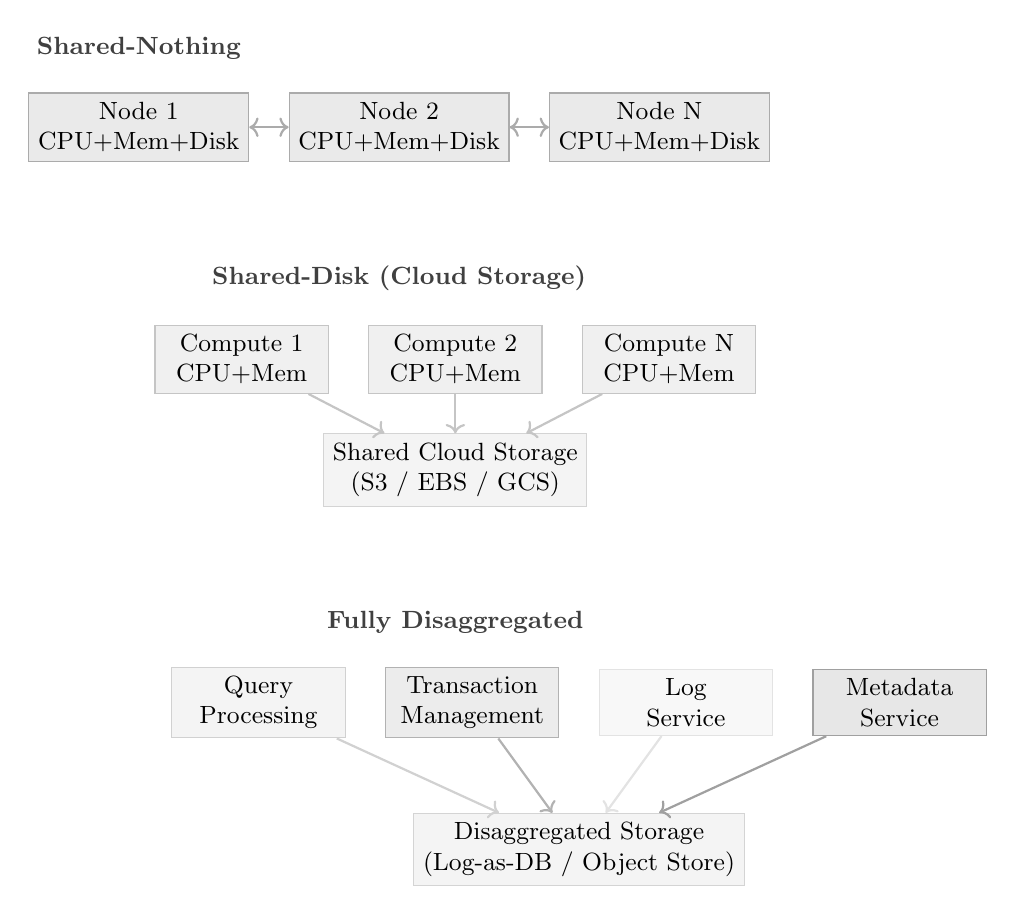
\begin{tikzpicture}[
    node distance=0.5cm and 2cm,
    box/.style={draw, minimum width=2.2cm, minimum height=0.8cm, font=\small, align=center, fill=#1!15, draw=#1!60},
    box/.default=cblue,
    arrow/.style={-{Stealth[length=3mm]}, thick, cdblue},
    label/.style={font=\small\bfseries, text=cdblue}
]

%% Shared-Nothing
\node[label] (sn_label) {Shared-Nothing};
\node[box=cblue, below=0.3cm of sn_label] (sn1) {Node 1\\CPU+Mem+Disk};
\node[box=cblue, right=0.5cm of sn1] (sn2) {Node 2\\CPU+Mem+Disk};
\node[box=cblue, right=0.5cm of sn2] (sn3) {Node N\\CPU+Mem+Disk};
\draw[<->, thick, cblue!60] (sn1) -- (sn2);
\draw[<->, thick, cblue!60] (sn2) -- (sn3);

%% Shared-Disk
\node[label, below=1.2cm of sn2] (sd_label) {Shared-Disk (Cloud Storage)};
\node[box=corange, below=0.3cm of sd_label, xshift=-2cm] (sd1) {Compute 1\\CPU+Mem};
\node[box=corange, right=0.5cm of sd1] (sd2) {Compute 2\\CPU+Mem};
\node[box=corange, right=0.5cm of sd2] (sd3) {Compute N\\CPU+Mem};
\node[box=cgray, below=0.5cm of sd2] (sd_storage) {Shared Cloud Storage\\(S3 / EBS / GCS)};
\draw[->, thick, corange!60] (sd1) -- (sd_storage);
\draw[->, thick, corange!60] (sd2) -- (sd_storage);
\draw[->, thick, corange!60] (sd3) -- (sd_storage);

%% Disaggregated
\node[label, below=1.2cm of sd_storage] (da_label) {Fully Disaggregated};
\node[box=cgreen, below=0.3cm of da_label, xshift=-2.5cm] (da_q) {Query\\Processing};
\node[box=cpurple, right=0.5cm of da_q] (da_t) {Transaction\\Management};
\node[box=cyellow, right=0.5cm of da_t] (da_l) {Log\\Service};
\node[box=cred, right=0.5cm of da_l] (da_m) {Metadata\\Service};
\node[box=cgray, below=1.4cm of $(da_t)!0.5!(da_l)$] (da_storage) {Disaggregated Storage\\(Log-as-DB / Object Store)};
\draw[->, thick, cgreen!60] (da_q) -- (da_storage);
\draw[->, thick, cpurple!60] (da_t) -- (da_storage);
\draw[->, thick, cyellow!60] (da_l) -- (da_storage);
\draw[->, thick, cred!60] (da_m) -- (da_storage);

\end{tikzpicture}
\caption{Evolution of cloud database architectures: from shared-nothing clusters to shared-disk (cloud storage) to fully disaggregated microservice architectures.}
\label{fig:architecture}
\end{figure}

\subsection{Data models in the cloud}
\label{subsec:datamodels}

Cloud platforms support a diverse ecosystem of data models, each optimized for different workload characteristics~\cite{Gessert2016NoSQL,Khasawneh2020SQLNewSQL,Han2011NoSQL,Tudorica2011NoSQLCmp,Bader2017TSDB,Ozsoyoglu1995Temporal}; early comparisons of the first-generation cloud stores such as SimpleDB and Bigtable already highlighted this model diversity~\cite{Ramanathan2011SimpleDBBigtable}. Table~\ref{tab:datamodels} compares the major data models available in cloud database services.

\begin{table}[H]
\centering
\caption{Cloud database data model landscape.}
\label{tab:datamodels}
\small
\begin{tabular}{p{2cm} p{2.5cm} p{3cm} p{4cm}}
\toprule
\textbf{Data Model} & \textbf{Strengths} & \textbf{Cloud Examples} & \textbf{Typical Use Cases} \\
\midrule
Relational & ACID, SQL, mature ecosystem & Aurora, Cloud SQL, Azure SQL & OLTP, ERP, financial systems \\
\addlinespace
Document & Schema flexibility, nested data & MongoDB Atlas, Cosmos DB, Firestore & Content management, catalogs, user profiles \\
\addlinespace
Key-Value & Ultra-low latency, high throughput & DynamoDB, Redis Cloud, Memorystore & Caching, session management, real-time \\
\addlinespace
Wide-Column & High write throughput, time-series & Bigtable, Cassandra (Astra), ScyllaDB & IoT, telemetry, event logging \\
\addlinespace
Graph & Relationship traversal, pattern matching & Neptune, Neo4j Aura, Cosmos DB (Gremlin) & Social networks, fraud detection, KGs \\
\addlinespace
Vector & Similarity search, ANN indexing & Pinecone, Weaviate, Milvus, pgvector & RAG, recommendation, image search \\
\addlinespace
Time-Series & Temporal queries, downsampling & TimescaleDB, InfluxDB Cloud, Timestream & Monitoring, financial ticks, sensor data \\
\addlinespace
Multi-Model & Multiple models in one engine & Cosmos DB, ArangoDB, SurrealDB & Polyglot persistence, unified access \\
\bottomrule
\end{tabular}
\end{table}

The trend toward \emph{multi-model databases}~\cite{Lu2019MultiModel} reflects the desire to avoid managing separate database systems for different data models. Azure Cosmos DB, for instance, supports document, graph, key-value, column-family, and table APIs through a single backend. However, multi-model integration introduces challenges in query optimization, consistency semantics, and performance trade-offs~\cite{Lu2019MultiModel}.

\subsection{The data platform continuum: warehouses, lakes, and lakehouses}
\label{subsec:continuum}

The cloud data management landscape has converged around three complementary paradigms, illustrated in Figure~\ref{fig:continuum}:

\begin{figure}[H]
\centering
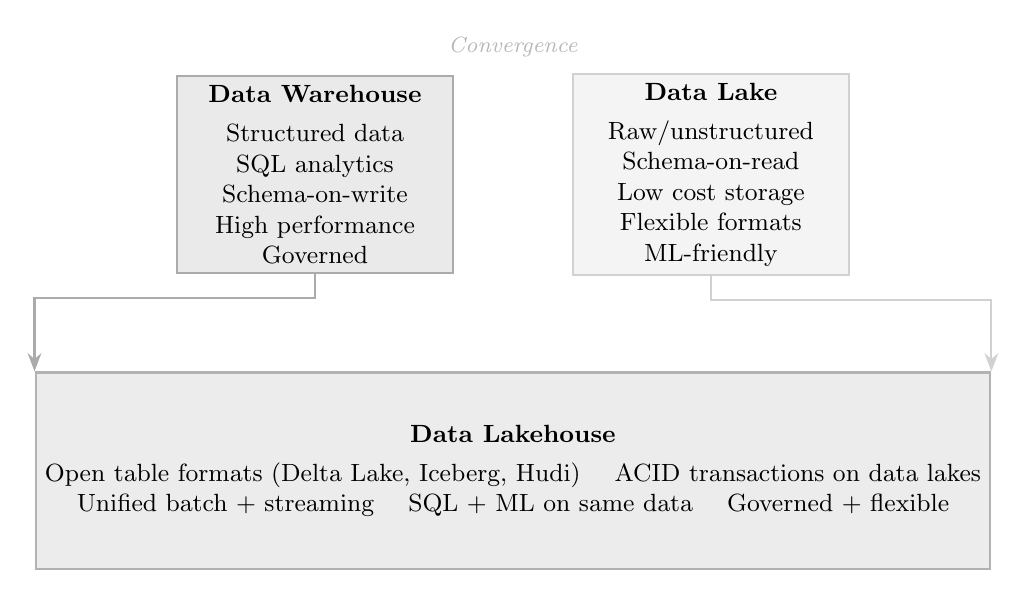
\begin{tikzpicture}[
    every node/.style={font=\small},
    box/.style={draw, minimum width=3.5cm, minimum height=2.5cm, align=center, thick}
]
%% Data Warehouse
\node[box, fill=cblue!15, draw=cblue!60] (dw) {
    \textbf{Data Warehouse}\\[3pt]
    Structured data\\
    SQL analytics\\
    Schema-on-write\\
    High performance\\
    Governed
};

%% Data Lake
\node[box, fill=cgreen!15, draw=cgreen!60, right=1.5cm of dw] (dl) {
    \textbf{Data Lake}\\[3pt]
    Raw/unstructured\\
    Schema-on-read\\
    Low cost storage\\
    Flexible formats\\
    ML-friendly
};

%% Data Lakehouse
\node[box, fill=cpurple!15, draw=cpurple!60, below=2.5cm of $(dw)!0.5!(dl)$, minimum width=8.5cm] (lh) {
    \textbf{Data Lakehouse}\\[3pt]
    Open table formats (Delta Lake, Iceberg, Hudi) \quad ACID transactions on data lakes\\
    Unified batch + streaming \quad SQL + ML on same data \quad Governed + flexible
};

%% Arrows
\draw[-{Stealth}, thick, cblue!60] (dw.south) -- ++(0,-0.3) -| (lh.north west);
\draw[-{Stealth}, thick, cgreen!60] (dl.south) -- ++(0,-0.3) -| (lh.north east);

%% Labels
\node[font=\footnotesize\itshape, text=cgray, above=0.1cm of $(dw.north)!0.5!(dl.north)$] {Convergence};
\end{tikzpicture}
\caption{The data platform continuum: data warehouses and data lakes converge into the data lakehouse paradigm.}
\label{fig:continuum}
\end{figure}

\textbf{Data warehouses} (e.g., Snowflake~\cite{Dageville2016}, BigQuery~\cite{Melnik2020Dremel}, Redshift) provide high-performance SQL analytics over structured, curated data with strong governance and schema enforcement.

\textbf{Data lakes} (e.g., Amazon S3 + Athena, Azure Data Lake Storage) offer cost-effective storage for raw, semi-structured, and unstructured data, enabling schema-on-read flexibility for data science and ML workloads.

\textbf{Data lakehouses}~\cite{Armbrust2021Lakehouse} combine the best of both paradigms by adding ACID transactions, schema enforcement, and data governance to open data lake storage through open table formats such as Delta Lake, Apache Iceberg, and Apache Hudi~\cite{Harby2022Lakehouse,Pohl2024LakehouseTS}.


%% ============================================================
%% SECTION 4: METHODOLOGY
%% ============================================================
\section{Systematic Review Planning and Execution}
\label{sec:methodology}

The systematic literature review (SLR) guidelines established by Kitchenham and Charters~\cite{Kitchenham2007}, which have been widely adopted in software engineering and computer science~\cite{Salehi2016Granular,Murtaza2020BreastCancer,Qazi2015SolarANN,Saeed2023XAI}, are followed. This protocol prescribes a three-phase process: (1)~\emph{planning}, in which research questions, search strategy, and inclusion/exclusion criteria are defined; (2)~\emph{conducting}, in which studies are systematically identified, selected, and their data extracted; and (3)~\emph{reporting}, in which the synthesized findings are documented and validated through quality assessment. The selection process is additionally reported using the PRISMA~2020 statement~\cite{Page2021PRISMA}, the de facto standard for transparent reporting of systematic reviews.


\subsection{Search strategy}
\label{subsec:searchstrategy}

The search was executed as a fully scripted, reproducible sweep over four scholarly indexing services via their public APIs on 5~July~2026, as detailed in Table~\ref{tab:searchterms}. OpenAlex and the arXiv API served as the primary sources; Crossref and Semantic Scholar were queried as supplementary sources to catch records missed by the primary indexes. The complete search scripts, the per-query result log, and every screening decision are archived alongside the manuscript (see the Data availability statement), so the identification stage can be re-executed verbatim.

\begin{table}[H]
\centering
\caption{Scholarly APIs searched (5~July~2026) and raw record yields. The OpenAlex sweep issued one query per cloud-database term (18 queries), each conjoined with the survey-indicator block of the canonical search string below; the arXiv sweep combined the \texttt{cs.DB} category with title-level survey indicators.}
\label{tab:searchterms}
\small
\begin{tabular}{p{3.4cm} p{6.2cm} r}
\toprule
\textbf{API} & \textbf{Query scope} & \textbf{Records} \\
\midrule
OpenAlex & Title + abstract; 18 term-queries $\times$ survey-indicator block; 1999--2026; article/review/preprint; English & 3,684 \\
arXiv API & \texttt{cat:cs.DB} $\times$ title survey-indicators & 356 \\
Crossref (suppl.) & Bibliographic relevance queries; journal articles from 1999 & 600 \\
Semantic Scholar (suppl.) & Bulk keyword search; 1999--2026 & 3,035 \\
\midrule
\multicolumn{2}{l}{Total raw records} & 7,675 \\
\multicolumn{2}{l}{After deduplication (DOI, arXiv id, normalized-title matching)} & 6,613 \\
\bottomrule
\end{tabular}
\end{table}

The canonical search string combines cloud database terminology with survey-indicating terms; it was applied natively by the OpenAlex queries and re-applied uniformly to all records (including the relevance-ranked supplementary sources) as an automated eligibility marking step:

\medskip
\noindent\fbox{\parbox{0.95\linewidth}{\small
\texttt{("cloud database" OR "cloud-native database" OR "DBaaS" OR "database-as-a-service" OR "serverless database" OR "HTAP" OR "NewSQL" OR "data lakehouse" OR "vector database" OR "AI4DB" OR "learned index" OR "NoSQL" OR "distributed database" OR "multi-model database" OR "graph database" OR "edge database" OR "fog database" OR "autonomous database")}\\
\texttt{AND}\\
\texttt{("survey" OR "review" OR "tutorial" OR "taxonomy" OR "systematic" OR "state-of-the-art" OR "overview")}
}}
\medskip

\subsection{Study selection}
\label{subsec:selection}

The inclusion and exclusion criteria listed in Table~\ref{tab:criteria} were applied in a two-phase process: (1)~title and abstract screening, and (2)~full-text assessment.

\begin{table}[H]
\centering
\caption{Inclusion and exclusion criteria.}
\label{tab:criteria}
\small
\begin{tabular}{c p{10cm}}
\toprule
\textbf{ID} & \textbf{Criterion} \\
\midrule
\multicolumn{2}{l}{\textit{Inclusion Criteria}} \\
IC1 & The paper is a survey, review, tutorial, or systematic mapping study \\
IC2 & The paper focuses primarily on cloud-hosted, cloud-native, or cloud-relevant database technologies \\
IC3 & The paper was published between January 1999 and the search date (July 2026) \\
IC4 & The paper is written in English \\
IC5 & The paper is peer-reviewed or published in a recognized venue (including arXiv with significant citations) \\
\addlinespace
\multicolumn{2}{l}{\textit{Exclusion Criteria}} \\
EC1 & The paper is a primary study (not a survey/review) \\
EC2 & The paper surveys cloud computing in general without database-specific focus \\
EC3 & The paper is a short paper ($<$6 pages) or workshop position paper \\
EC4 & The paper is a duplicate or substantially overlapping earlier version \\
EC5 & The full text could not be retrieved (no open-access copy and no manually obtainable copy) \\
\bottomrule
\end{tabular}
\end{table}

\subsection{Quality assessment}
\label{subsec:quality}

Each candidate survey was evaluated against eight quality assessment criteria (QA1--QA8), scored on a 3-point scale (0 = No, 0.5 = Partially, 1 = Yes). Given the breadth of the expanded 1999--2026 identification pool, the inclusion threshold was set at 6 out of 8; papers scoring below this threshold were excluded (papers scoring between 4 and 6 are reported explicitly in the selection flow).

\begin{table}[H]
\centering
\caption{Quality assessment checklist for surveyed papers.}
\label{tab:qa}
\small
\begin{tabular}{c p{10cm}}
\toprule
\textbf{ID} & \textbf{Quality Assessment Question} \\
\midrule
QA1 & Are the survey objectives clearly stated? \\
QA2 & Is the scope and coverage of the survey well-defined? \\
QA3 & Is the search/selection methodology described or implied? \\
QA4 & Does the survey provide a taxonomy or classification framework? \\
QA5 & Are the reviewed primary studies adequately described? \\
QA6 & Does the survey identify open challenges or future directions? \\
QA7 & Is the survey published in a recognized venue (journal, top conference, or high-citation arXiv)? \\
QA8 & Is the survey sufficiently comprehensive ($\geq$30 references)? \\
\bottomrule
\end{tabular}
\end{table}

\subsection{Results: study selection and demographics}
\label{subsec:results}

Figure~\ref{fig:prisma} presents the PRISMA~2020 flow diagram of the selection process, with two identification arms: records identified through the scripted database search, and records identified through other methods (the previous version of this catalog, manually collected reports, and backward snowballing). From 7,675 raw database records, 96 surveys were ultimately included in the meta-survey.

\begin{figure}[H]
\centering
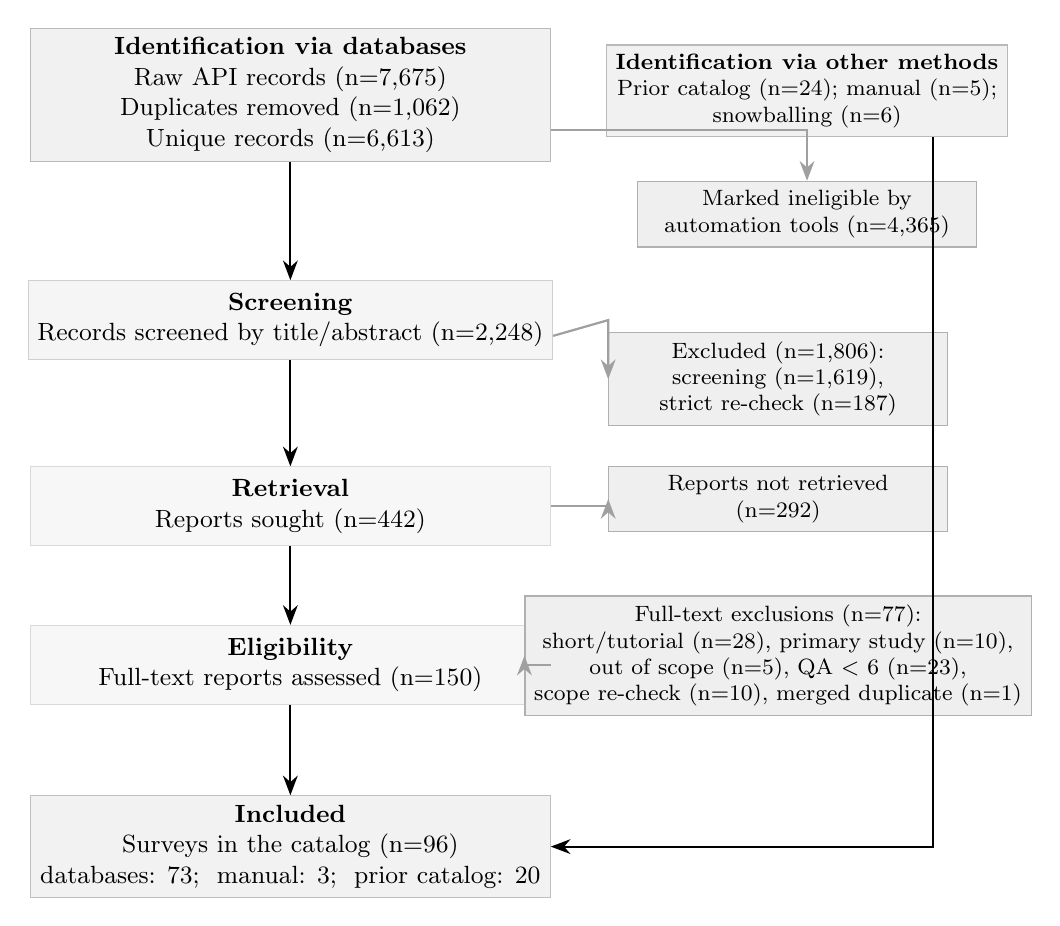
\begin{tikzpicture}[
    node distance=0.8cm,
    box/.style={draw, minimum width=6.6cm, minimum height=1cm, align=center, font=\small, fill=#1!10, draw=#1!50},
    box/.default=cblue,
    sbox/.style={draw, minimum width=4.6cm, minimum height=0.9cm, align=center, font=\footnotesize, fill=#1!10, draw=#1!50},
    sbox/.default=cblue,
    arrow/.style={-{Stealth[length=2.5mm]}, thick},
    excl/.style={draw, minimum width=4.3cm, minimum height=0.8cm, align=center, font=\footnotesize, fill=cred!10, draw=cred!50}
]

\node[box=cblue] (id) {\textbf{Identification via databases}\\Raw API records (n=7{,}675)\\Duplicates removed (n=1{,}062)\\Unique records (n=6{,}613)};
\node[sbox=cblue, right=0.7cm of id, yshift=0.05cm] (oth) {\textbf{Identification via other methods}\\Prior catalog (n=24); manual (n=5);\\snowballing (n=6)};
\node[excl, below=0.55cm of oth] (autoex) {Marked ineligible by\\automation tools (n=4{,}365)};
\node[box=corange, below=1.5cm of id] (sc) {\textbf{Screening}\\Records screened by title/abstract (n=2{,}248)};
\node[excl, right=0.7cm of sc, yshift=-0.75cm] (ex1) {Excluded (n=1{,}806):\\screening (n=1{,}619),\\strict re-check (n=187)};
\node[box=cgreen, below=1.35cm of sc] (el) {\textbf{Retrieval}\\Reports sought (n=442)};
\node[excl, below=0.5cm of ex1] (ex2) {Reports not retrieved\\(n=292)};
\node[box=cgreen, below=1cm of el] (ft) {\textbf{Eligibility}\\Full-text reports assessed (n=150)};
\node[excl, below=0.8cm of ex2] (ex3) {Full-text exclusions (n=77):\\short/tutorial (n=28), primary study (n=10),\\out of scope (n=5), QA $<$ 6 (n=23),\\scope re-check (n=10), merged duplicate (n=1)};
\node[box=cpurple, below=1.15cm of ft] (inc) {\textbf{Included}\\Surveys in the catalog (n=96)\\databases: 73;~~manual: 3;~~prior catalog: 20};

\draw[arrow] (id) -- (sc);
\draw[arrow] (sc) -- (el);
\draw[arrow] (el) -- (ft);
\draw[arrow] (ft) -- (inc);
\draw[arrow, cred!60] (id.east) ++(0,-0.45) -| (autoex.north);
\draw[arrow, cred!60] (sc.east) ++(0,-0.2) -- (ex1.west |- sc.east) -- (ex1.west);
\draw[arrow, cred!60] (el.east) -- (ex2.west |- el.east) -- (ex2.west);
\draw[arrow, cred!60] (ft.east) -- (ex3.west |- ft.east) -- (ex3.west);
\draw[arrow] (oth.south) ++(1.6,0) |- (inc.east);

\end{tikzpicture}
\caption{PRISMA~2020 flow diagram of the study selection process~\cite{Page2021PRISMA}. All figures are scripted tallies over the archived screening-decision log. The full-text exclusion box aggregates one merged duplicate of a prior-catalog entry; of the six snowball candidates, one was retrieved and excluded below the quality threshold and five could not be retrieved. Two prior-catalog entries failed the raised quality threshold and were removed.}
\label{fig:prisma}
\end{figure}

Figure~\ref{fig:byyear} shows the distribution of selected surveys by publication year. Survey activity is sparse before 2016, grows steadily through the late 2010s, and intensifies markedly from 2024 onward---2024 and 2025 together account for more than a third of the corpus.

\begin{figure}[H]
\centering
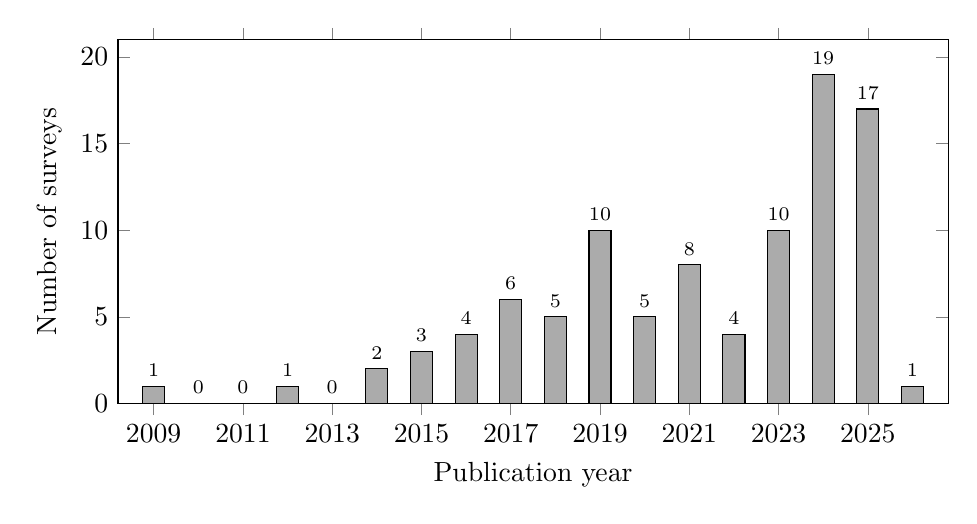
\begin{tikzpicture}
\begin{axis}[
    ybar,
    bar width=0.28cm,
    width=\linewidth,
    height=6.2cm,
    ylabel={Number of surveys},
    xlabel={Publication year},
    xmin=2008.2, xmax=2026.8,
    xtick={2009,2011,2013,2015,2017,2019,2021,2023,2025},
    xticklabel style={/pgf/number format/1000 sep=},
    ymin=0,
    ymax=21,
    nodes near coords,
    nodes near coords align={vertical},
    every node near coord/.append style={font=\scriptsize, text=black},
]
\addplot[fill=cblue!60, draw=black] coordinates {(2009,1) (2010,0) (2011,0) (2012,1) (2013,0) (2014,2) (2015,3) (2016,4) (2017,6) (2018,5) (2019,10) (2020,5) (2021,8) (2022,4) (2023,10) (2024,19) (2025,17) (2026,1)};
\end{axis}
\end{tikzpicture}
\caption{Distribution of the 96 selected surveys by publication year. Although the search window opens in January 1999, the earliest survey satisfying all inclusion and quality criteria dates from 2009; the 2026 bar covers only the months up to the search date (July 2026).}
\label{fig:byyear}
\end{figure}

Figure~\ref{fig:bytopic} shows the distribution by primary topic domain (each survey is assigned a single primary topic, so the counts sum to 96). NoSQL/NewSQL systems are the most frequently surveyed topic, reflecting the maturity and breadth of that body of literature, followed by graph databases and AI4DB/learned database components.

\begin{figure}[H]
\centering
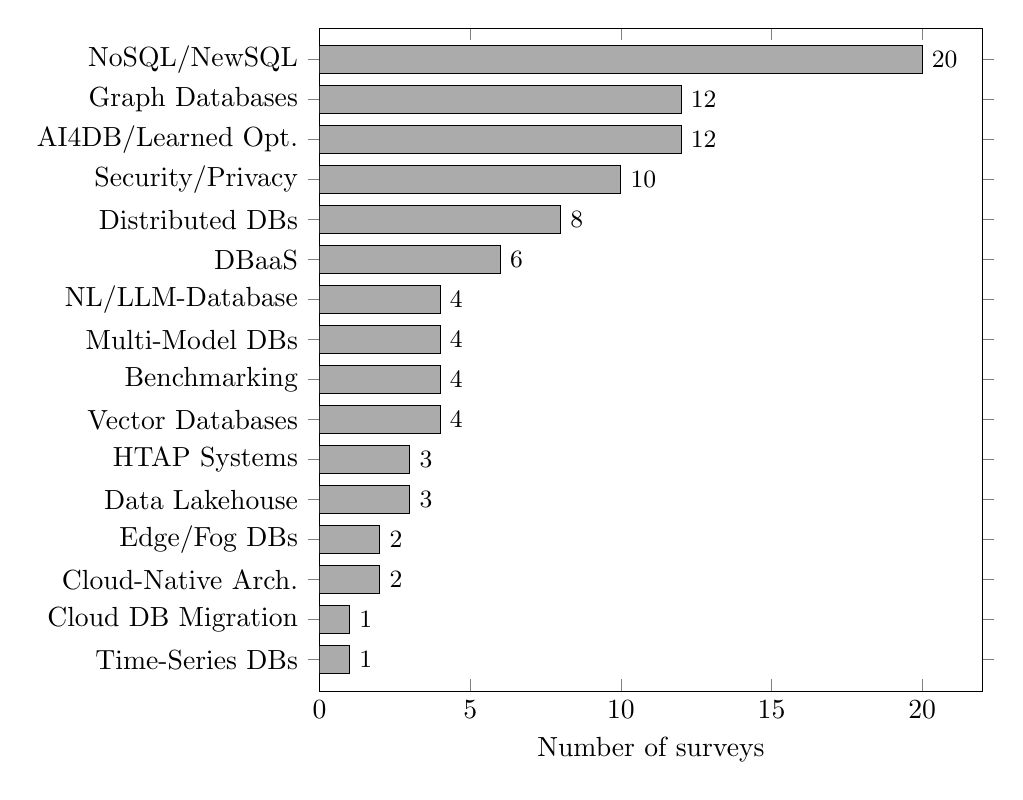
\begin{tikzpicture}
\begin{axis}[
    xbar,
    bar width=0.35cm,
    width=10cm,
    height=10cm,
    xlabel={Number of surveys},
    xmin=0,
    xmax=22,
    ytick=data,
    symbolic y coords={
        {Time-Series DBs},
        {Cloud DB Migration},
        {Cloud-Native Arch.},
        {Edge/Fog DBs},
        {Data Lakehouse},
        {HTAP Systems},
        {Vector Databases},
        {Benchmarking},
        {Multi-Model DBs},
        {NL/LLM-Database},
        {DBaaS},
        {Distributed DBs},
        {Security/Privacy},
        {AI4DB/Learned Opt.},
        {Graph Databases},
        {NoSQL/NewSQL}
    },
    nodes near coords,
    nodes near coords align={horizontal},
    every node near coord/.append style={font=\small, text=black},
    enlarge y limits={abs=0.4cm},
]
\addplot[fill=cblue!60, draw=black] coordinates {
    (20,{NoSQL/NewSQL})
    (12,{Graph Databases})
    (12,{AI4DB/Learned Opt.})
    (10,{Security/Privacy})
    (8,{Distributed DBs})
    (6,{DBaaS})
    (4,{NL/LLM-Database})
    (4,{Multi-Model DBs})
    (4,{Benchmarking})
    (4,{Vector Databases})
    (3,{HTAP Systems})
    (3,{Data Lakehouse})
    (2,{Edge/Fog DBs})
    (2,{Cloud-Native Arch.})
    (1,{Cloud DB Migration})
    (1,{Time-Series DBs})
};
\end{axis}
\end{tikzpicture}
\caption{Distribution of the 96 selected surveys by primary topic domain.}
\label{fig:bytopic}
\end{figure}

Figure~\ref{fig:byvenue} shows the distribution by venue type. Journal publications account for the majority, followed by arXiv preprints and conference proceedings; the visible arXiv share reflects both the field's preprint culture and the open-access retrieval policy described in Section~\ref{subsec:threats}.

\begin{figure}[H]
\centering
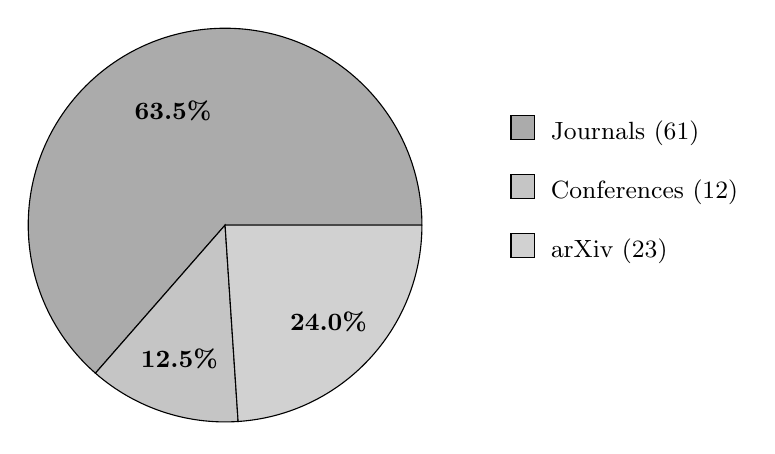
\begin{tikzpicture}
  %% Pie chart drawn manually with TikZ (counts from the frozen catalog.csv;
  %% angles generated by search/generate_catalog_artifacts.py).
  %% Journals (61): 63.5% = 228.8 deg, Conferences (12): 12.5% = 45 deg, arXiv (23): 24.0% = 86.2 deg
  \def\radius{2.5}

  %% Slice 1: Journals (0 to 228.8)
  \filldraw[fill=cblue!60, draw=black, thin] (0,0) -- (0:\radius) arc (0:228.8:\radius) -- cycle;
  \node at (114.4:1.6) {\small\textbf{63.5\%}};

  %% Slice 2: Conferences (228.8 to 273.8)
  \filldraw[fill=corange!60, draw=black, thin] (0,0) -- (228.8:\radius) arc (228.8:273.8:\radius) -- cycle;
  \node at (251.2:1.8) {\small\textbf{12.5\%}};

  %% Slice 3: arXiv (273.8 to 360)
  \filldraw[fill=cgreen!60, draw=black, thin] (0,0) -- (273.8:\radius) arc (273.8:360:\radius) -- cycle;
  \node at (316.9:1.8) {\small\textbf{24.0\%}};

  %% Legend
  \node[anchor=west] at (3.5, 1.2) {\small\tikz\filldraw[fill=cblue!60,draw=black] (0,0) rectangle (0.3,0.3); \;Journals (61)};
  \node[anchor=west] at (3.5, 0.45) {\small\tikz\filldraw[fill=corange!60,draw=black] (0,0) rectangle (0.3,0.3); \;Conferences (12)};
  \node[anchor=west] at (3.5, -0.3) {\small\tikz\filldraw[fill=cgreen!60,draw=black] (0,0) rectangle (0.3,0.3); \;arXiv (23)};
\end{tikzpicture}
\caption{Distribution of the 96 selected surveys by venue type.}
\label{fig:byvenue}
\end{figure}

\subsection{Threats to validity}
\label{subsec:threats}

As with any systematic review, this meta-survey is subject to validity threats, which are mitigated as follows.

\textbf{Construct validity.} The search string and the choice of indexing services may not capture every relevant survey, particularly those using non-standard terminology or absent from the OpenAlex, arXiv, Crossref, and Semantic Scholar indexes; abstract availability in these indexes is also uneven, which affects the automated eligibility marking. These threats are mitigated by (i)~running fully scripted queries whose logs are archived and re-executable, (ii)~taking the union of four independent APIs rather than relying on a single index, (iii)~carrying forward the previous version of the catalog as a separate identification arm, and (iv)~a backward-snowballing pass over the reference lists of the highest-scoring included surveys, which surfaced no additional qualifying survey---evidence that the search had reached saturation. The English-language filter may exclude relevant surveys in other languages.

\textbf{Internal validity.} Study selection, quality assessment, and data extraction were performed by a single reviewer, introducing a risk of subjective bias and a lack of inter-rater agreement. To reduce this threat, explicit inclusion/exclusion criteria (Table~\ref{tab:criteria}) and a documented quality-assessment rubric (Table~\ref{tab:qa}) were applied uniformly, and borderline decisions were re-examined in a second pass. Every included survey was additionally verified against a resolvable DOI or arXiv identifier and a retained full-text copy, so that the catalog contains only confirmable publications. The absence of a second independent reviewer nonetheless remains a limitation.

\textbf{External validity.} As a survey of surveys, the findings inherit the scope and currency limitations of the primary surveys; rapidly evolving topics (e.g., LLM--database convergence) may be underrepresented relative to their current activity. The corpus is further subject to an open-access retrieval bias: every included survey must have a content-verified full text on file, and 292 otherwise-eligible reports could not be retrieved through any open-access channel (reported explicitly in the PRISMA flow), so paywalled surveys---particularly from the early 2000s---are underrepresented. Notably, no survey published before 2009 satisfied all criteria, so the 1999--2008 portion of the window is represented in the narrative (Section~\ref{subsec:history}) rather than the catalog. The synthesis is therefore intended as a structured map of the field rather than an exhaustive account of every primary system.

\textbf{Conclusion validity.} The challenge taxonomy and the consensus/divergence synthesis (Table~\ref{tab:challenge-synthesis}) involve interpretive judgment. These are grounded in explicit per-challenge evidence and cross-referenced to the surveyed domains in Table~\ref{tab:challenge-coverage} to keep the reasoning traceable.


%% ============================================================
%% SECTION 5: DISCUSSION
%% ============================================================
\section{Discussion---Challenges and Research Directions}
\label{sec:discussion}

This section presents the core contribution of this meta-survey: a comprehensive, structured analysis of the challenges and research directions identified across the 96 surveyed papers. Following the dual-theme approach of Saeed and Omlin~\cite{Saeed2023XAI}, the discussion is organized into two complementary themes:

\begin{enumerate}
    \item \textbf{Theme~1: Cross-cutting challenges} (Section~\ref{subsec:theme1})---eighteen recurring challenges that transcend individual system categories.
    \item \textbf{Theme~2: Lifecycle-phase challenges} (Section~\ref{subsec:theme2})---challenges organized by the five phases of the cloud database lifecycle.
\end{enumerate}

Figure~\ref{fig:taxonomy} provides a high-level overview of the dual-theme taxonomy.

\begin{figure}[t]
\centering
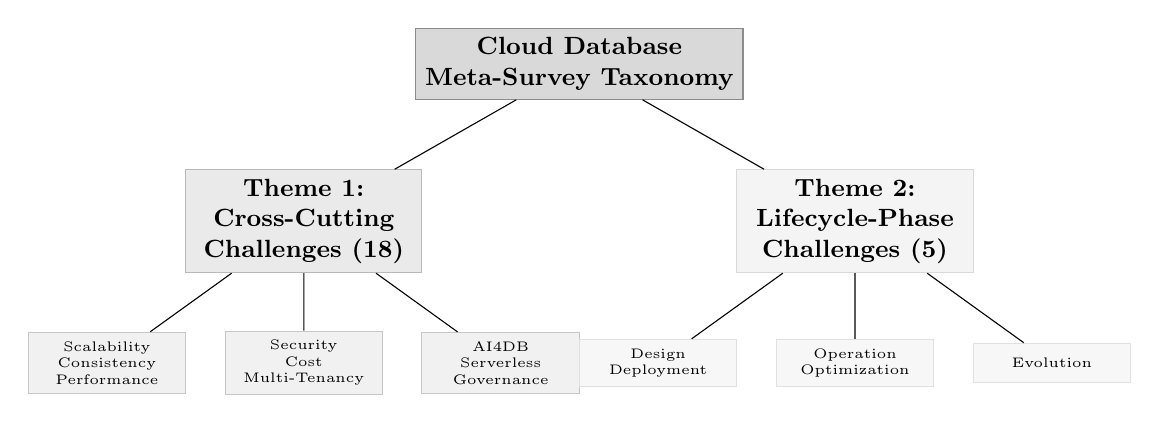
\begin{tikzpicture}[
    level 1/.style={sibling distance=7cm, level distance=2cm},
    level 2/.style={sibling distance=2.5cm, level distance=1.8cm},
    root/.style={draw, fill=cdblue!20, draw=cdblue!60, font=\small\bfseries, minimum width=4cm, minimum height=0.8cm, align=center},
    theme/.style={draw, fill=#1!15, draw=#1!50, font=\small\bfseries, minimum width=3cm, minimum height=0.7cm, align=center},
    leaf/.style={draw, fill=#1!10, draw=#1!40, font=\tiny, minimum width=2cm, minimum height=0.5cm, align=center},
]

\node[root] {Cloud Database\\Meta-Survey Taxonomy}
    child {node[theme=cblue] {Theme 1:\\Cross-Cutting\\Challenges (18)}
        child {node[leaf=cblue] {Scalability\\Consistency\\Performance}}
        child {node[leaf=cblue] {Security\\Cost\\Multi-Tenancy}}
        child {node[leaf=cblue] {AI4DB\\Serverless\\Governance}}
    }
    child {node[theme=cgreen] {Theme 2:\\Lifecycle-Phase\\Challenges (5)}
        child {node[leaf=cgreen] {Design\\Deployment}}
        child {node[leaf=cgreen] {Operation\\Optimization}}
        child {node[leaf=cgreen] {Evolution}}
    };

\end{tikzpicture}
\caption{High-level taxonomy of the cloud database meta-survey, organized into two complementary themes.}
\label{fig:taxonomy}
\end{figure}

\subsection{Theme 1: Cross-cutting challenges}
\label{subsec:theme1}

Eighteen cross-cutting challenges that recur across multiple cloud database survey domains are identified and organized, in Figure~\ref{fig:challenge-fanout}, into four clusters---\emph{foundational}, \emph{data-architecture}, \emph{operational}, and \emph{emerging} concerns. Each challenge is discussed as a short narrative that frames the problem, summarizes the current state reported across the surveyed papers (including points of consensus and divergence), and closes with a brief statement of the open problems and research directions---highlighting data- and knowledge-engineering (DKE) relevance---that the surveys leave unresolved.

\begin{figure}[t]
\centering
\adjustbox{max width=\linewidth}{%
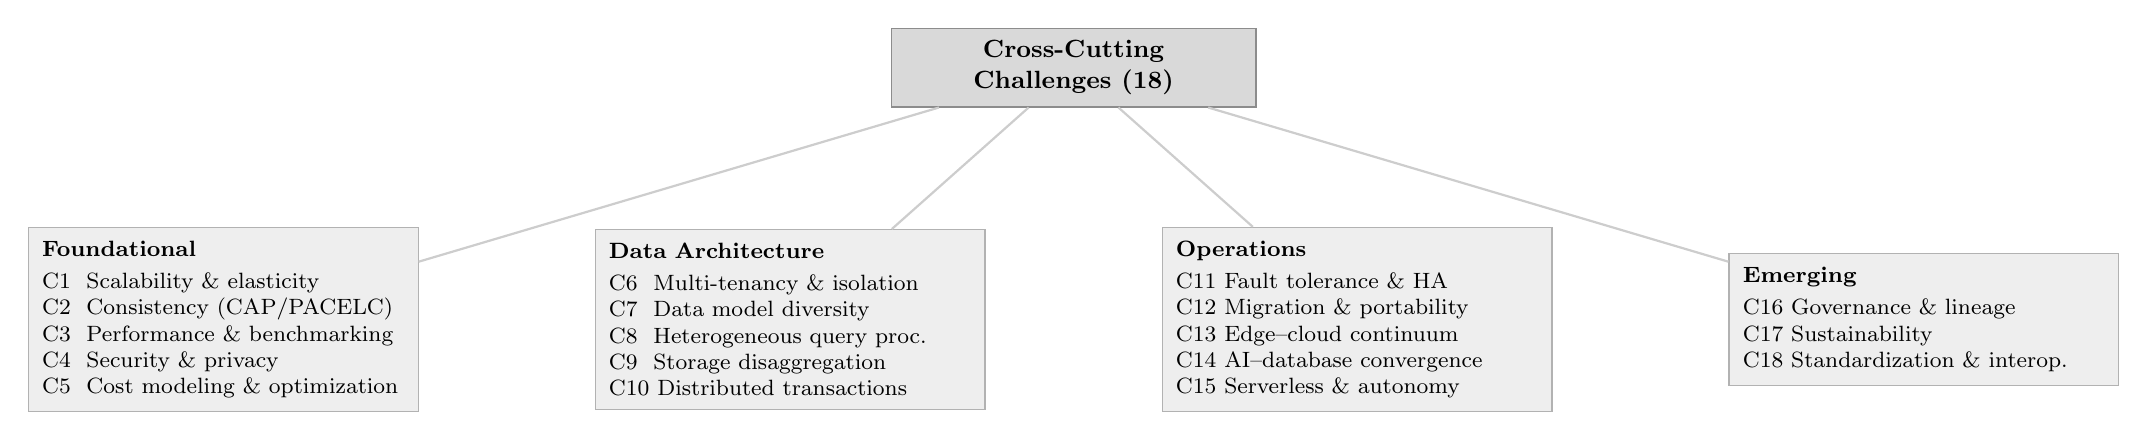
\begin{tikzpicture}[
  root/.style={draw, fill=cdblue!20, draw=cdblue!60, font=\small\bfseries, align=center, minimum height=1.0cm, text width=4.4cm},
  clu/.style={draw, fill=cblue!12, draw=cblue!55, font=\footnotesize, align=left, text width=4.6cm, inner sep=5pt},
  spoke/.style={-, thick, cgray!70}
]
\node[root] (r) at (0,3.2) {Cross-Cutting\\Challenges (18)};
\node[clu] (f) at (-10.8,0) {\textbf{Foundational}\\[2pt] C1~~Scalability \& elasticity\\ C2~~Consistency (CAP/PACELC)\\ C3~~Performance \& benchmarking\\ C4~~Security \& privacy\\ C5~~Cost modeling \& optimization};
\node[clu] (d) at (-3.6,0) {\textbf{Data Architecture}\\[2pt] C6~~Multi-tenancy \& isolation\\ C7~~Data model diversity\\ C8~~Heterogeneous query proc.\\ C9~~Storage disaggregation\\ C10~Distributed transactions};
\node[clu] (o) at (3.6,0) {\textbf{Operations}\\[2pt] C11~Fault tolerance \& HA\\ C12~Migration \& portability\\ C13~Edge--cloud continuum\\ C14~AI--database convergence\\ C15~Serverless \& autonomy};
\node[clu] (e) at (10.8,0) {\textbf{Emerging}\\[2pt] C16~Governance \& lineage\\ C17~Sustainability\\ C18~Standardization \& interop.};
\draw[spoke] (r) -- (f);
\draw[spoke] (r) -- (d);
\draw[spoke] (r) -- (o);
\draw[spoke] (r) -- (e);
\end{tikzpicture}}
\caption{The eighteen cross-cutting challenges, organized into four clusters.}
\label{fig:challenge-fanout}
\end{figure}

Three consolidated views support the discussion. Table~\ref{tab:challenge-coverage} maps each challenge to the survey domains that address it, revealing coverage density and thematic clusters; Table~\ref{tab:challenge-synthesis} synthesizes the key points of agreement and divergence across surveyed papers; and Table~\ref{tab:challenge-year} shows how attention to each challenge has evolved over the study window. Detailed discussion follows in Sections~\ref{subsubsec:scalability}--\ref{subsubsec:standardization}.

%% ---- Table 1: Challenge Coverage Matrix ----
\begin{landscape}
\setlength{\LTcapwidth}{\linewidth}
\begin{small}
\begin{longtable}{c >{\raggedright\arraybackslash}p{3.0cm} *{14}{c} r}
\caption{Cross-cutting challenge coverage across consolidated survey domains. Symbols: \FULL~=~primary focus, \PART~=~substantive discussion, \MINOR~=~mentioned. The rightmost column~(\textit{n}) counts domains addressing each challenge.}
\label{tab:challenge-coverage}\\
\toprule
\# & Challenge & \rot{Cloud-Native} & \rot{HTAP} & \rot{NoSQL / NewSQL} & \rot{AI4DB / Learned} & \rot{Vector / Graph / Multi-Model} & \rot{Lakehouse} & \rot{Time-Series} & \rot{Edge / Fog} & \rot{NL / LLM--DB} & \rot{Security / Privacy} & \rot{Benchmarking} & \rot{Migration} & \rot{Distributed DBs} & \rot{DBaaS} & \textit{n} \\
\midrule
\endfirsthead
\multicolumn{17}{l}{\small\textit{Table~\ref{tab:challenge-coverage} continued}}\\
\toprule
\# & Challenge & \rot{Cloud-Native} & \rot{HTAP} & \rot{NoSQL / NewSQL} & \rot{AI4DB / Learned} & \rot{Vector / Graph / Multi-Model} & \rot{Lakehouse} & \rot{Time-Series} & \rot{Edge / Fog} & \rot{NL / LLM--DB} & \rot{Security / Privacy} & \rot{Benchmarking} & \rot{Migration} & \rot{Distributed DBs} & \rot{DBaaS} & \textit{n} \\
\midrule
\endhead
\midrule
\multicolumn{17}{r}{\small\textit{Continued on next page}}\\
\endfoot
\bottomrule
\endlastfoot
%% Foundational
\multicolumn{17}{l}{\textit{Foundational}}\\
\addlinespace
C1  & Scalability \& elasticity          & \FULL & \PART & \FULL  & \MINOR &        & \PART & \PART & \PART &       &       & \PART &       & \PART & \PART & 10 \\
C2  & Consistency \& CAP/PACELC          & \FULL & \FULL & \FULL  &        & \MINOR &       &       & \PART &       &       &       &       & \FULL &  & 6 \\
C3  & Performance \& benchmarking        & \FULL & \PART & \PART  & \FULL  &        & \PART &       &       &       &       & \FULL &       & \PART &  & 7 \\
C4  & Security \& privacy                & \PART &       & \MINOR &        &        &       &       & \PART &       & \FULL &       & \MINOR &  & \PART & 6 \\
C5  & Cost modeling \& optimization      & \PART &       &        &        &        & \PART &       &       &       &       & \FULL & \PART &  & \PART & 5 \\
\addlinespace
%% Data Architecture
\multicolumn{17}{l}{\textit{Data Architecture}}\\
\addlinespace
C6  & Multi-tenancy \& isolation         & \FULL &       &        &        &        &       &       &       &       & \PART & \PART &       &  & \FULL & 4 \\
C7  & Data model diversity               &       & \MINOR & \FULL &        & \FULL  & \PART & \PART &       &       &       &       &       &  &  & 5 \\
C8  & Heterogeneous query processing     & \PART & \FULL & \MINOR & \PART  & \PART  & \FULL &       &       & \PART &       &       &       & \PART &  & 8 \\
C9  & Storage disaggregation             & \FULL & \PART &        &        &        & \FULL &       &       &       &       &       &       &  &  & 4 \\
C10  & Distributed transactions           & \FULL & \FULL & \FULL  &        & \MINOR &       &       & \MINOR &      &       &       &       & \FULL &  & 5 \\
\addlinespace
%% Operations
\multicolumn{17}{l}{\textit{Operations}}\\
\addlinespace
C11  & Fault tolerance \& HA              & \FULL &       & \PART  &        &        &       &       & \PART &       &       &       &       & \FULL &  & 4 \\
C12  & Migration \& portability           & \PART &       & \MINOR &        &        &       &       &       &       &       &       & \FULL &  & \PART & 4 \\
C13  & Edge--cloud continuum              & \MINOR &      &        &        &        &       &       & \FULL &       & \MINOR &      &       &  &  & 3 \\
C14  & AI--database convergence           & \PART &       &        & \FULL  & \MINOR & \PART &       &       & \FULL &       &       &       &  &  & 5 \\
C15  & Serverless \& autonomy             & \FULL &       &        & \PART  &        &       &       &       &       &       & \MINOR &       &  & \PART & 4 \\
\addlinespace
%% Emerging
\multicolumn{17}{l}{\textit{Emerging}}\\
\addlinespace
C16  & Governance \& lineage              & \MINOR &      &        &        &        & \PART &       &       & \MINOR & \FULL &      & \MINOR &  & \MINOR & 5 \\
C17  & Sustainability                     & \MINOR &      &        & \MINOR &        &       &       &       &       &       & \PART &       &  &  & 3 \\
C18  & Standardization \& interoperability & \PART &      & \PART  &        & \FULL  & \PART &       &       & \MINOR &      &       & \PART & \MINOR &  & 7 \\
\end{longtable}
\end{small}
\end{landscape}

%% ---- Table 2: Synthesis of Similarities and Differences ----
\begin{landscape}
\setlength{\LTcapwidth}{\linewidth}
\begin{small}
\begin{longtable}{c >{\raggedright\arraybackslash}p{2.2cm} >{\raggedright\arraybackslash}p{2.5cm} >{\raggedright\arraybackslash}p{7.2cm} >{\raggedright\arraybackslash}p{7.2cm}}
\caption{Synthesis of cross-cutting challenges: key similarities (consensus) and differences (divergences) across the 96 surveyed papers, referenced at survey-domain granularity (domain sizes as in Figure~\ref{fig:bytopic}).}
\label{tab:challenge-synthesis}\\
\toprule
\# & Challenge & Survey domains (\textit{n}) & Key Similarities (Consensus) & Key Differences (Divergences) \\
\midrule
\endfirsthead
\multicolumn{5}{l}{\small\textit{Table~\ref{tab:challenge-synthesis} continued}}\\
\toprule
\# & Challenge & Survey domains (\textit{n}) & Key Similarities (Consensus) & Key Differences (Divergences) \\
\midrule
\endhead
\midrule
\multicolumn{5}{r}{\small\textit{Continued on next page}}\\
\endfoot
\bottomrule
\endlastfoot
%% Foundational
C1 & Scalability \& elasticity &
49 surveys in Cloud-Native, HTAP, NoSQL/NewSQL, Lakehouse, Time-Series, Edge/Fog, Benchmarking, Distributed DBs, DBaaS &
All surveys agree that disaggregated storage enables elastic scaling; horizontal scale-out is preferred over vertical scaling; auto-scaling is a baseline cloud capability. &
Cloud-native surveys focus on component-level elasticity; NoSQL surveys emphasize partition-based data scaling; HTAP surveys and edge/fog surveys stress elasticity under mixed and intermittently connected workloads, respectively. \\
\addlinespace
C2 & Consistency \& CAP/PACELC &
35 surveys in Cloud-Native, HTAP, NoSQL/NewSQL, Edge/Fog, Distributed DBs &
CAP/PACELC trade-offs are universally acknowledged; all surveys recognize a spectrum from strong to eventual consistency; configurable consistency is a key cloud differentiator. &
NoSQL surveys accept eventual consistency as pragmatic; HTAP surveys insist on strong consistency for transactional correctness; cloud-native surveys present tunable consistency as an application-level choice. \\
\addlinespace
C3 & Performance \& benchmarking &
52 surveys in Cloud-Native, HTAP, NoSQL/NewSQL, AI4DB/Learned, Lakehouse, Benchmarking, Distributed DBs &
Cloud-specific factors (network latency, multi-tenancy, cold starts) complicate optimization; existing benchmarks (TPC-C/H, YCSB) are widely considered inadequate for cloud settings. &
AI4DB surveys emphasize learned optimizers and indexes; benchmarking surveys focus on measurement methodology and fairness; cloud-native surveys focus on disaggregation overhead. \\
\addlinespace
C4 & Security \& privacy &
20 surveys in Cloud-Native, Edge/Fog, Security/Privacy, DBaaS &
Encryption at rest and in transit is a baseline requirement; the shared responsibility model is universally acknowledged; GDPR compliance is a common concern. &
Security surveys deeply analyze threat models and advanced techniques (homomorphic encryption, confidential computing); cloud-native surveys treat security as one concern among many; edge/fog surveys emphasize privacy-preserving aggregation. \\
\addlinespace
C5 & Cost modeling \& optimization &
16 surveys in Cloud-Native, Lakehouse, Benchmarking, Migration, DBaaS &
Cost is a primary driver of cloud adoption; pricing complexity (10--100$\times$ variation) is widely noted; pay-per-use models are a defining benefit. &
Benchmarking surveys focus on total cost of ownership comparison; lakehouse surveys weigh storage--compute cost trade-offs; migration surveys highlight hidden migration and lock-in costs; cloud-native surveys note multi-dimensional pricing complexity. \\
\addlinespace
%% Data Architecture
C6 & Multi-tenancy \& isolation &
22 surveys in Cloud-Native, Security/Privacy, Benchmarking, DBaaS &
Noisy-neighbor performance interference is universally recognized; the trade-off between resource sharing efficiency and isolation is a fundamental tension. &
Cloud-native surveys focus on architectural isolation levels (shared-nothing to shared-table); security surveys emphasize tenant data isolation; benchmarking surveys measure interference under controlled conditions. \\
\addlinespace
C7 & Data model diversity &
44 surveys in NoSQL/NewSQL, Vector/Graph/Multi-Model, Lakehouse, Time-Series &
Polyglot persistence is the operational reality; cross-model query support is needed; multi-model databases are gaining traction. &
NoSQL surveys favor model-specific optimization; multi-model surveys advocate unified backends; specialized surveys argue that model-native operations (vector, graph, time-series) cannot be efficiently reduced to a single backend. \\
\addlinespace
C8 & Heterogeneous query processing &
52 surveys in Cloud-Native, HTAP, AI4DB/Learned, Vector/Graph/Multi-Model, Lakehouse, NL/LLM--DB, Distributed DBs &
Federated query processing across engines is increasingly necessary; predicate pushdown is the baseline optimization technique. &
HTAP surveys focus on OLTP--OLAP workload routing; lakehouse surveys emphasize open-format access layers; multi-model surveys and natural-language interface surveys address cross-model and intent-driven query routing. \\
\addlinespace
C9 & Storage disaggregation &
28 surveys in Cloud-Native, HTAP, Lakehouse, NoSQL/NewSQL &
Compute-storage separation is the defining cloud-native architectural principle; write amplification reduction is a key benefit; independent layer scaling is a primary motivation. &
Cloud-native surveys focus on log-as-database architectures (Aurora, PolarDB); lakehouse surveys emphasize open table formats; HTAP surveys address separate analytical and transactional storage tiers. \\
\addlinespace
C10 & Distributed transactions &
33 surveys in Cloud-Native, HTAP, NoSQL/NewSQL, Distributed DBs &
2PC and consensus protocols (Paxos/Raft) are the dominant approaches; the consistency--latency trade-off is universally acknowledged. &
Cloud-native surveys cite clock synchronization innovations (TrueTime, HLC); NoSQL surveys accept weaker guarantees (CRDTs, eventual consistency); HTAP surveys focus on OLTP--OLAP transaction isolation. \\
\addlinespace
%% Operations
C11 & Fault tolerance \& HA &
32 surveys in Cloud-Native, NoSQL/NewSQL, Edge/Fog, Distributed DBs &
Multi-AZ replication is the baseline approach; automated failover is expected; RTO/RPO targets drive architectural decisions. &
Cloud-native surveys focus on quorum protocols (e.g., Aurora's 4/6 write quorum); NoSQL surveys emphasize tunable replication factors; edge/fog surveys must handle intermittent connectivity. \\
\addlinespace
C12 & Migration \& portability &
9 surveys in Cloud-Native, Migration, DBaaS &
Migration is complex, error-prone, and labor-intensive; schema heterogeneity is the primary technical barrier; vendor lock-in is widely criticized. &
Migration surveys focus on methodology and zero-downtime techniques; cloud-native surveys treat migration as a cloud adoption path; NoSQL surveys highlight data model mismatch challenges. \\
\addlinespace
C13 & Edge--cloud continuum &
2 surveys in Edge/Fog &
Data placement across edge--fog--cloud tiers requires intelligent policies; intermittent connectivity is the defining constraint. &
Edge/fog surveys focus on resource-constrained processing and synchronization; cloud-native surveys view edge as a cloud extension; security surveys emphasize privacy-preserving edge aggregation. \\
\addlinespace
C14 & AI--database convergence &
21 surveys in Cloud-Native, AI4DB/Learned, Lakehouse, NL/LLM--DB &
Both AI4DB and DB4AI directions are growing rapidly; production deployment of learned components remains limited; training data management is a shared challenge. &
AI4DB surveys focus on individual learned components (indexes, optimizers); natural-language and retrieval-augmented surveys address LLM-driven querying and retrieval; cloud-native surveys view AI as a system enhancement. \\
\addlinespace
C15 & Serverless \& autonomy &
20 surveys in Cloud-Native, AI4DB/Learned, DBaaS &
Serverless abstracts infrastructure management; cold-start latency is a known limitation; pay-per-query suits variable workloads. &
Cloud-native surveys treat serverless as one deployment model and catalog autoscaling mechanisms; AI4DB surveys envision full-stack autonomous databases that self-tune beyond the serverless abstraction. \\
\addlinespace
%% Emerging
C16 & Governance \& lineage &
13 surveys in Lakehouse, Security/Privacy &
End-to-end lineage tracking is increasingly important; regulatory compliance (GDPR, CCPA) drives governance adoption; metadata management is fragmented across tools. &
Security surveys focus on access control and audit logging; lakehouse surveys emphasize unified data cataloging; migration surveys track lineage across system transitions; cloud-native and NL-interface surveys note metadata's role in querying. \\
\addlinespace
C17 & Sustainability &
4 surveys in Benchmarking &
Energy-proportional computing is an aspirational goal; carbon-aware data placement is an emerging research direction. &
Cloud-native surveys note the energy implications of disaggregation; AI4DB surveys flag the training cost of learned components; benchmarking surveys propose adding energy and carbon metrics; most other survey domains do not yet address sustainability. \\
\addlinespace
C18 & Standardization \& interoperability &
46 surveys in Cloud-Native, NoSQL/NewSQL, Vector/Graph/Multi-Model, Lakehouse, Migration &
Vendor lock-in is widely criticized; SQL remains the primary query lingua franca; open formats (Iceberg, Delta Lake, Hudi) are gaining traction. &
Graph and specialized surveys highlight query-language fragmentation (Cypher, SPARQL, GQL); NoSQL surveys focus on API heterogeneity; multi-model and natural-language interface surveys push unified access, while migration surveys stress portable formats. \\
\end{longtable}
\end{small}
\end{landscape}

%% ---- Table: temporal attention heatmap (challenge x year) ----
\begin{landscape}
\setlength{\LTcapwidth}{\linewidth}
\begin{small}
\begin{longtable}{c >{\raggedright\arraybackslash}p{4.6cm} *{5}{c} c}
\caption{Temporal attention to each cross-cutting challenge: the number of surveyed papers, by publication period, whose primary domain substantively (\FULL/\PART) addresses the challenge. Cell shading is scaled within each row; attention concentrates in 2023--2026, mirroring the overall publication trend (Figure~\ref{fig:byyear}).}
\label{tab:challenge-year}\\
\toprule
\# & Challenge & 2009--2015 & 2016--2019 & 2020--2022 & 2023--2024 & 2025--2026 & Total \\
\midrule
\endfirsthead
\multicolumn{8}{l}{\small\textit{Table~\ref{tab:challenge-year} continued}}\\
\toprule
\# & Challenge & 2009--2015 & 2016--2019 & 2020--2022 & 2023--2024 & 2025--2026 & Total \\
\midrule
\endhead
\midrule
\multicolumn{8}{r}{\small\textit{Continued on next page}}\\
\endfoot
\bottomrule
\endlastfoot
C1 & Scalability \& elasticity & \cellcolor{cgray!36}4 & \cellcolor{cgray!60}10 & \cellcolor{cgray!64}11 & \cellcolor{cgray!80}15 & \cellcolor{cgray!56}9 & 49 \\
C2 & Consistency \& CAP/PACELC & \cellcolor{cgray!38}3 & \cellcolor{cgray!56}6 & \cellcolor{cgray!74}9 & \cellcolor{cgray!80}10 & \cellcolor{cgray!62}7 & 35 \\
C3 & Performance \& benchmarking & \cellcolor{cgray!31}3 & \cellcolor{cgray!50}8 & \cellcolor{cgray!65}12 & \cellcolor{cgray!80}16 & \cellcolor{cgray!68}13 & 52 \\
C4 & Security \& privacy & \cellcolor{cgray!50}3 & \cellcolor{cgray!80}6 & \cellcolor{cgray!50}3 & \cellcolor{cgray!70}5 & \cellcolor{cgray!50}3 & 20 \\
C5 & Cost modeling \& optimization & \cellcolor{cgray!30}1 & \cellcolor{cgray!60}4 & \cellcolor{cgray!40}2 & \cellcolor{cgray!80}6 & \cellcolor{cgray!50}3 & 16 \\
C6 & Multi-tenancy \& isolation & \cellcolor{cgray!50}3 & \cellcolor{cgray!80}6 & \cellcolor{cgray!50}3 & \cellcolor{cgray!80}6 & \cellcolor{cgray!60}4 & 22 \\
C7 & Data model diversity & \cellcolor{cgray!32}3 & \cellcolor{cgray!67}11 & \cellcolor{cgray!62}10 & \cellcolor{cgray!80}14 & \cellcolor{cgray!45}6 & 44 \\
C8 & Heterogeneous query processing & \cellcolor{cgray!26}2 & \cellcolor{cgray!64}14 & \cellcolor{cgray!38}6 & \cellcolor{cgray!80}19 & \cellcolor{cgray!54}11 & 52 \\
C9 & Storage disaggregation & \cellcolor{cgray!33}2 & \cellcolor{cgray!40}3 & \cellcolor{cgray!80}9 & \cellcolor{cgray!80}9 & \cellcolor{cgray!53}5 & 28 \\
C10 & Distributed transactions & \cellcolor{cgray!40}3 & \cellcolor{cgray!60}6 & \cellcolor{cgray!73}8 & \cellcolor{cgray!80}9 & \cellcolor{cgray!66}7 & 33 \\
C11 & Fault tolerance \& HA & \cellcolor{cgray!42}3 & \cellcolor{cgray!65}6 & \cellcolor{cgray!80}8 & \cellcolor{cgray!80}8 & \cellcolor{cgray!72}7 & 32 \\
C12 & Migration \& portability & \cellcolor{cgray!35}1 & \cellcolor{cgray!80}4 &   & \cellcolor{cgray!50}2 & \cellcolor{cgray!50}2 & 9 \\
C13 & Edge--cloud continuum &   &   & \cellcolor{cgray!80}1 & \cellcolor{cgray!80}1 &   & 2 \\
C14 & AI--database convergence &   & \cellcolor{cgray!54}4 & \cellcolor{cgray!45}3 & \cellcolor{cgray!80}7 & \cellcolor{cgray!80}7 & 21 \\
C15 & Serverless \& autonomy & \cellcolor{cgray!28}1 & \cellcolor{cgray!62}5 & \cellcolor{cgray!37}2 & \cellcolor{cgray!62}5 & \cellcolor{cgray!80}7 & 20 \\
C16 & Governance \& lineage & \cellcolor{cgray!50}2 & \cellcolor{cgray!65}3 & \cellcolor{cgray!65}3 & \cellcolor{cgray!80}4 & \cellcolor{cgray!35}1 & 13 \\
C17 & Sustainability &   &   & \cellcolor{cgray!50}1 & \cellcolor{cgray!80}2 & \cellcolor{cgray!50}1 & 4 \\
C18 & Standardization \& interop. & \cellcolor{cgray!32}3 & \cellcolor{cgray!64}11 & \cellcolor{cgray!60}10 & \cellcolor{cgray!80}15 & \cellcolor{cgray!48}7 & 46 \\
\midrule
\multicolumn{2}{l}{\textbf{Total (challenge-mentions)}} & \textbf{37} & \textbf{107} & \textbf{101} & \textbf{153} & \textbf{100} & \textbf{498} \\
\end{longtable}
\end{small}
\end{landscape}

\subsubsection{Scalability and elasticity}
\label{subsubsec:scalability}

Scalability---handling growing workloads by adding resources---and elasticity---provisioning and releasing resources in response to demand---are the foundational promises of the cloud, and every surveyed cloud-native and NoSQL review treats them as first-order concerns~\cite{Li2024CloudNativeSurvey,Davoudian2018NoSQL}; efforts to quantify elasticity empirically date back to the first wave of cloud data stores~\cite{Dory2011Elasticity}. In practice, cloud-native engines such as Aurora~\cite{Verbitski2017} and Snowflake~\cite{Dageville2016} achieve storage elasticity through compute--storage disaggregation, while compute elasticity is delivered by auto-scaling and replication~\cite{Thara2013DaaSPerf}; serverless offerings push this further by scaling to zero between requests~\cite{Muller2020Serverless}. The surveyed literature nonetheless converges on a shared limitation: today's elasticity is coarse-grained, operating at the level of whole instances rather than individual components, so that \emph{fine-grained} elasticity---independently scaling a single query operator, the transaction manager, or the log service---remains largely unrealized~\cite{Li2024CloudNativeSurvey}.

Several obstacles recur across the reviews. Cold-start latency undermines the responsiveness that makes scale-to-zero attractive~\cite{Muller2020Serverless}; state migration during scale-out and scale-in introduces transient performance degradation; and predictive autoscaling depends on workload-forecasting models that are still maturing~\cite{Ma2021LearnedWorkload}. Cross-component elasticity in fully disaggregated architectures is the least understood of all, because the interactions among independently scaled layers are difficult to model.

\textbf{Open problems and research directions.} The central open problem is a principled account of \emph{elastic data architectures} that links workload patterns, resource allocation, performance guarantees, and cost. From a data- and knowledge-engineering standpoint, ontological models of cloud-database configurations and their scaling behavior could turn today's heuristic autoscaling into reasoning over an explicit model, enabling predictable, component-level elasticity.

\subsubsection{Consistency, availability, and partition tolerance revisited}
\label{subsubsec:consistency}

The CAP theorem~\cite{Brewer2012CAP} and its PACELC refinement~\cite{Abadi2012PACELC} have shaped distributed database design for over a decade, but the surveyed work shows that geo-distribution, multi-region deployment, and the proliferation of configurable consistency levels give these trade-offs new dimensions in the cloud~\cite{Viotti2016Consistency}. Cloud databases now expose a spectrum of guarantees: Spanner provides external consistency via TrueTime~\cite{Corbett2013Spanner}, whereas systems such as Cosmos DB offer several intermediate levels from strong to eventual. Surveys of NoSQL stores~\cite{Davoudian2018NoSQL,Kaur2021NoSQLReview} and of HTAP systems~\cite{Haas2024HTAPSurvey} consistently single out consistency management as a defining difficulty, and they disagree on how much weakening is acceptable---NoSQL reviews accept eventual consistency as pragmatic, while HTAP and NewSQL reviews insist on strong guarantees for transactional correctness.

What the surveys leave open is largely a matter of reasoning and tooling. Developers struggle to predict how a given consistency level affects application correctness~\cite{Viotti2016Consistency}; adaptive consistency that adjusts to workload requirements is frequently proposed but rarely deployed; and cross-model consistency---reconciling, say, document and graph views of the same data---is barely studied in multi-model settings~\cite{Lu2019MultiModel}.

\textbf{Open problems and research directions.} Bridging the gap between formal consistency models and everyday development calls for knowledge-based specifications of consistency \emph{contracts}---machine-checkable statements of the guarantees a service offers and an application requires---so that compatibility can be verified rather than assumed, a natural fit for formal-methods and DKE techniques.

\subsubsection{Performance optimization and benchmarking}
\label{subsubsec:performance}

Performance optimization in the cloud spans query optimization, indexing, caching, resource allocation, and workload management, and benchmarking supplies the empirical ground truth against which systems are compared~\cite{Rabl2019BenchmarkSurvey}. The AI4DB and cloud-native reviews document substantial progress on the optimization side---learned query optimization~\cite{Marcus2021Bao}, learned indexes~\cite{Kraska2018LearnedIndex}, and automated knob tuning~\cite{Zhang2022CDBTune}---yet they emphasize that cloud-specific factors such as network latency, disaggregation overhead, multi-tenant interference, and cold starts confound techniques designed for single-node systems~\cite{Zhou2022AI4DB,Li2024CloudNativeSurvey}. On the measurement side, the benchmarking reviews are unanimous that classical benchmarks (TPC-C, TPC-H, YCSB) fail to capture cloud realities such as elasticity, pay-per-use pricing, and variable network performance~\cite{Rabl2019BenchmarkSurvey,Taipalus2024DBMSPerf,Samarta2024SQLNoSQL,Daundasekara2025MultiCloud}.

The unresolved issues follow directly. Cloud-aware benchmarks that incorporate elasticity, multi-tenancy, and pricing are still lacking; fair cross-provider comparison is confounded by differing hardware, pricing, and service-level agreements; and end-to-end performance in disaggregated stacks emerges from complex interactions among independently scaled layers that no current benchmark isolates.

\textbf{Open problems and research directions.} A promising direction is a \emph{benchmark knowledge base} that formally records configurations, workload characteristics, hardware, and results in a structured, queryable representation; making benchmark provenance explicit would render cloud-database evaluations reproducible and genuinely comparable---an evaluation problem with a strong knowledge-engineering core.

\subsubsection{Security and privacy}
\label{subsubsec:security}

Relative to on-premises systems, cloud databases face an enlarged attack surface arising from shared infrastructure, network-based access, and the need to trust the provider~\cite{Fuhrt2010CloudSecurity,Zubi2009DistSec,Waghmare2015CloudDBSec}. The security-focused surveys catalog the established defenses---encryption at rest and in transit, access control, audit logging, and vulnerability management~\cite{Sanka2022CloudSecSurvey,Ferrari2009DBaaSSec,Munir2015DBaaSSec,Khan2019DaaSAnalytic}---and the more advanced techniques that target computation over protected data, including homomorphic encryption for querying ciphertext~\cite{Acar2018HE,Ravan2013EncQuery}, architectures giving clients distributed, concurrent access to encrypted cloud databases without a trusted broker~\cite{Ferretti2014Encrypted}, private-database models for outsourced data~\cite{Cuzzocrea2016PrivateDB}, secure multi-party computation, and confidential computing in hardware enclaves. The reviews differ in emphasis: dedicated security surveys analyze threat models in depth, whereas cloud-native reviews treat security as one concern among many and edge-oriented work stresses privacy-preserving aggregation close to the data source.

Across the literature the same hard problems persist: the performance overhead of encryption remains prohibitive for analytics; key management across multi-cloud and hybrid deployments is error-prone; the ``honest but curious'' provider is difficult to defend against without heavy penalties; and reconciling GDPR's right to erasure with analytic utility is unsolved.

\textbf{Open problems and research directions.} \emph{Privacy ontologies} that formally model data sensitivity, access policies, and regulatory obligations would let compliance be checked and enforced automatically across heterogeneous cloud deployments, turning today's manual, document-driven compliance into machine-reasoned policy---squarely a DKE contribution.

\subsubsection{Cost modeling and optimization}
\label{subsubsec:cost}

Cloud databases bill along many dimensions at once---compute hours, storage, I/O operations, network egress, backups, and premium features such as encryption or multi-region replication---which makes cost both a primary adoption driver and a persistent source of surprise~\cite{Leis2023CloudPricing}. Empirical studies show that the cost of the same workload can vary by one to two orders of magnitude depending on configuration~\cite{Leis2023CloudPricing}, and although work on serverless analytics~\cite{Muller2020Serverless} and the cloud-native reviews~\cite{Li2024CloudNativeSurvey} flag cost as critical, they offer little quantitative guidance. The benchmarking and migration reviews add the complementary observations that total-cost-of-ownership comparison and hidden lock-in costs are rarely modeled rigorously~\cite{Taipalus2024DBMSPerf,Mathew2021CloudMigration}.

Consequently, pre-execution cost estimation for complex analytical queries remains unreliable; multi-objective optimization over cost, performance, and consistency lacks mature frameworks; the trade-offs among reserved, on-demand, and spot capacity for database workloads are understudied; and vendor lock-in obscures cross-provider comparison.

\textbf{Open problems and research directions.} Formal \emph{cost knowledge models}---ontologies that capture provider pricing structures, workload profiles, and optimization strategies---could support automated, explainable cost optimization, and would give the field a shared vocabulary for reasoning about cloud economics rather than per-provider spreadsheets.

\subsubsection{Multi-tenancy and resource isolation}
\label{subsubsec:multitenancy}

Multi-tenancy lets providers serve many customers from shared infrastructure, improving utilization and lowering cost, at the price of harder performance isolation, data separation, and fair resource allocation~\cite{Li2024CloudNativeSurvey}. The surveyed systems realize tenancy at several granularities---shared-nothing (an instance per tenant), shared-process (logical isolation within one engine), and shared-table (row-level security over common tables)---and the reviews repeatedly identify ``noisy neighbor'' interference, in which one tenant's load degrades another's latency, as the dominant operational hazard~\cite{Narasayya2015MultiTenant}.

\textbf{Open problems and research directions.} Achieving strong performance isolation without dedicating hardware remains difficult; workload-aware scheduling that adapts to heterogeneous tenants is immature; and the fundamental tension between sharing efficiency and isolation guarantees still lacks a principled, cost-aware resolution. Quantitative models that predict interference from tenant workload signatures are a promising avenue.

\subsubsection{Data model diversity and multi-model integration}
\label{subsubsec:multimodel}

The cloud has multiplied the data models in routine use---relational, document, graph, key-value, wide-column, vector, and time-series---and applications increasingly need to query across several at once~\cite{Lu2019MultiModel,Jain2016HighVariety,Baralis2017Geospatial,Mahmood2019NoSQLLog}. Multi-model engines such as Cosmos DB, ArangoDB, and SurrealDB expose multiple model interfaces over a single backend, and the NoSQL and multi-model surveys report growing adoption alongside a candid account of the limits: cross-model query optimization and unified transaction semantics remain weak~\cite{Davoudian2018NoSQL,Tu2024CassandraMongo,Hendricks2019NoSQLReview,Tripathi2025NoSQLEdu,Lu2019MultiModel}. The reviews also diverge on strategy---NoSQL surveys favor model-specific optimization, multi-model surveys advocate unified backends, and specialized reviews argue that vector, graph, and time-series operations cannot be reduced efficiently to a single engine.

\textbf{Open problems and research directions.} The persistent gaps are unified query languages spanning relational, graph, document, and vector operations; cross-model optimization of queries that combine, say, graph traversal with relational joins and similarity search; and schema mapping across models. Using ontologies to provide a single conceptual layer over diverse physical models---\emph{knowledge representation for multi-model data}---is a direct DKE opportunity.

\subsubsection{Query processing across heterogeneous engines}
\label{subsubsec:queryprocessing}

Modern cloud data stacks rarely rely on a single engine; OLTP, OLAP, graph, search, and vector systems must be queried in concert, making federated query processing and data virtualization essential~\cite{Haas2024HTAPSurvey,Sheng2025MQRLD}. Engines such as Presto/Trino, BigQuery Omni, and AWS Lake Formation already provide federation, and the HTAP reviews analyze how queries should be routed to the appropriate engine~\cite{Haas2024HTAPSurvey}; yet they agree that cross-engine optimization is still rudimentary, seldom going beyond predicate pushdown. The unresolved problems are cost-based optimization across engines with incompatible cost models and capabilities, preserving transactional guarantees across engine boundaries, and the semantic understanding of data needed to route queries intelligently rather than syntactically.

\textbf{Open problems and research directions.} \emph{Ontology-mediated query answering}~\cite{Xiao2018OBDA} offers a principled basis for posing a single query against many heterogeneous engines through a shared conceptual schema, connecting cloud query federation to a long line of DKE research on data integration.

\subsubsection{Storage disaggregation and log-as-database}
\label{subsubsec:disaggregation}

Separating compute from storage into independently scalable layers is the defining architectural move of the cloud-native era, and the ``log-as-database'' pattern pioneered by Aurora---treating the redo log itself as the system of record---pushes intelligence into the storage tier~\cite{Verbitski2017,Li2024CloudNativeSurvey}. This design reduced write amplification and enabled fast failover, and systems such as PolarDB~\cite{Cao2021PolarDB} and Socrates~\cite{Antonopoulos2019} carry disaggregation further by splitting out additional components. The cloud-native surveys report that while disaggregation simplifies operations and scaling, it introduces its own difficulties in remote-I/O latency, cache coherence, and log management~\cite{Li2024CloudNativeSurvey}.

\textbf{Open problems and research directions.} Outstanding issues include masking the latency gap between remote storage and local SSDs, coordinating caches across compute and storage layers, and managing the log at scale through compaction, garbage collection, and efficient replay. Cost- and latency-aware models of where computation should run within a disaggregated stack are a promising research direction.

\subsubsection{Transaction processing in distributed cloud environments}
\label{subsubsec:transactions}

Distributed transaction processing must balance ACID guarantees against performance and scalability, and the surveyed systems span the full design space from strongly consistent protocols (two-phase commit, Paxos/Raft) to relaxed models such as CRDTs and eventual consistency~\cite{Corbett2013Spanner,Taft2020Cockroach}. Spanner demonstrated that globally distributed, strongly consistent transactions are feasible using synchronized clocks~\cite{Corbett2013Spanner}, and CockroachDB and YugabyteDB provide comparable guarantees with hybrid logical clocks~\cite{Taft2020Cockroach}; the NewSQL and HTAP reviews nonetheless report that sustaining strong consistency at high throughput for mixed workloads is still hard~\cite{Haas2024HTAPSurvey}.

\textbf{Open problems and research directions.} The recurring open problems are reducing commit latency for geo-distributed transactions without weakening consistency, resolving conflicts efficiently across regions, and isolating transactional and analytical work within a single HTAP engine so that neither degrades the other.

\subsubsection{Fault tolerance, recovery, and high availability}
\label{subsubsec:faulttolerance}

Cloud databases must survive hardware faults, network partitions, availability-zone outages, and even whole-region failures while preserving durability and minimizing downtime~\cite{Verbitski2017,Li2024CloudNativeSurvey}. The prevailing approach is multi-availability-zone replication---typically three-way---with automated failover, exemplified by Aurora's six-replica, three-zone write quorum~\cite{Verbitski2017}. The surveys report that recovery-time objectives of seconds and near-zero recovery-point objectives are attainable within a single region, but remain difficult to guarantee across regions.

\textbf{Open problems and research directions.} Multi-region disaster recovery with near-zero RPO and RTO is still open, as is consistent recovery in disaggregated architectures whose state is scattered across components; the surveyed work also notes the absence of chaos-engineering and fault-injection frameworks tailored to cloud databases, which would let resilience be tested systematically rather than anecdotally.

\subsubsection{Data migration and cross-cloud portability}
\label{subsubsec:migration}

Organizations routinely move databases between on-premises and cloud, between providers, and between services, and the migration survey documents how hard it is to preserve consistency, minimize downtime, and transform schemas along the way~\cite{Mathew2021CloudMigration}. Although every major provider offers a migration service, the reviewed evidence is that migrations remain error-prone and labor-intensive, with schema and data-model mismatches the principal technical barrier and vendor lock-in---through proprietary APIs, formats, and features---compounding the difficulty of any subsequent move~\cite{Opara2017LockIn}.

\textbf{Open problems and research directions.} The field still lacks zero-downtime migration for large, continuously written databases, automated schema mapping between heterogeneous systems, and portability layers that abstract provider-specific features. \emph{Knowledge-based schema mapping}, which represents schema semantics ontologically to automate translation, ties cloud migration directly to DKE's long-standing strengths in schema integration and data exchange.

\subsubsection{Edge--cloud data continuum}
\label{subsubsec:edgecloud}

The spread of IoT devices, autonomous vehicles, and smart-city infrastructure has created demand for database capability at the network edge operating in concert with the cloud~\cite{Gomes2024EdgeFog}, a pressure recognized early in evaluations of cloud databases for IoT data~\cite{Phan2014IoTCloudDB}. The edge-and-fog survey maps architectures that distribute storage and query processing across edge devices, fog nodes, and cloud backends, and notes that systems such as Azure SQL Edge, AWS Outposts, and locality-aware features in CockroachDB address only parts of the problem~\cite{Gomes2024EdgeFog}.

\textbf{Open problems and research directions.} Maintaining consistency across the edge--fog--cloud continuum under intermittent connectivity, deciding intelligently which data to cache, replicate, or move, processing queries under tight resource constraints on edge devices, and aggregating data privately before it reaches the cloud all remain open. Policy models that reason about placement against latency, privacy, and connectivity constraints are a promising direction.

\subsubsection{AI--database convergence (AI4DB and DB4AI)}
\label{subsubsec:ai4db}

The convergence of AI and databases runs in two directions---AI4DB, which uses learning to optimize the database, and DB4AI, which uses database technology to serve AI workloads~\cite{Zhou2022AI4DB}. The AI4DB surveys document concrete progress in learned query optimization~\cite{Marcus2021Bao}, learned indexes~\cite{Kraska2018LearnedIndex,Zhao2026SpatialIndex,Woltmann2023DNNIndex}, automated knob and buffer tuning~\cite{Zhang2022CDBTune,Tan2019iBTune}, learned partitioning advisors~\cite{Hilprecht2020Partitioning}, cardinality estimation, and workload forecasting~\cite{Ma2021LearnedWorkload,Dritsas2026MLDB}, while DB4AI spans in-database machine learning and optimized data serving for training pipelines. The reviews agree that learned components are rarely yet trusted in production, and that managing their training data is a shared, unsolved concern. The persistent obstacles are deploying learned components with safety guarantees so that they degrade gracefully when a model fails, collecting and curating training data from live workloads, transferring learned behavior across instances and hardware, and---perhaps most important for adoption---explaining why a learned optimizer made a given decision.

\textbf{Open problems and research directions.} \emph{Knowledge engineering for self-driving databases}, which couples explicit domain knowledge about database internals with learned models, is a promising route to autonomous systems that are both robust and explainable---an agenda where DKE and the database community meet directly.

\subsubsection{Serverless and autonomous database operations}
\label{subsubsec:serverless}

Serverless databases hide infrastructure entirely, provisioning, scaling, patching, and tuning without operator involvement, and autonomous databases go further by using machine learning to self-diagnose and self-heal~\cite{Pavlo2017SelfDriving,Muller2020Serverless}. Offerings such as Aurora Serverless v2, the Cosmos DB serverless tier, Neon, and PlanetScale realize the serverless interface, while Oracle Autonomous Database is the most ambitious autonomy effort; studies of serverless data systems report that the model suits variable workloads well but struggles with sustained high throughput and cold-start latency~\cite{Muller2020Serverless}.

\textbf{Open problems and research directions.} Predictable performance under serverless autoscaling, transparent exposure of the cost--performance trade-off, and full-stack autonomy that unifies self-tuning, self-healing, and self-securing remain open. The cloud-native and AI4DB reviews converge on the view that genuine autonomy will require databases to reason about their own behavior, not merely react---again pointing to a knowledge-grounded approach.

\subsubsection{Data governance, provenance, and lineage}
\label{subsubsec:governance}

As cloud data ecosystems grow, tracking where data came from (provenance), how it was transformed (lineage), and whether its use complies with policy becomes essential for compliance, debugging, and trust~\cite{Halevy2016Goods}. The governance-related surveys identify a common set of needs---metadata management, data cataloging, access control, quality monitoring, and regulatory compliance---and report that cloud-native tools such as AWS Glue Data Catalog, Azure Purview, and Google Dataplex address them only partially, leaving the landscape fragmented and unstandardized. The unresolved problems are end-to-end lineage that spans heterogeneous services and processing engines, automated checking against regulatory requirements that themselves keep changing, and provenance-aware query processing that records how each result was derived.

\textbf{Open problems and research directions.} Representing and linking metadata as a \emph{knowledge graph} over cloud data assets, and reasoning over it, is a natural DKE contribution that would unify cataloging, lineage, and compliance under a single queryable model.

\subsubsection{Sustainability and energy efficiency}
\label{subsubsec:sustainability}

Data centers consumed an estimated 1--1.5\% of global electricity in 2023, with projections of 3--4\% by 2030 as AI and cloud workloads grow, and cloud databases---heavy consumers of compute and storage---contribute directly to that footprint~\cite{IEA2024DataCenters}. Work on green computing identifies opportunities in energy-efficient query processing, scheduling that follows renewable-energy availability, and carbon-aware data placement; major providers now report carbon metrics, but the surveyed evidence is that database-level energy optimization is still nascent.

\textbf{Open problems and research directions.} Energy-proportional databases that consume resources in line with actual load, carbon-aware placement and replication that favor cleaner grids, and benchmarks that report energy and carbon alongside performance are the principal open directions; sustainability is also the least-addressed challenge across the surveyed domains, marking it as an opportunity rather than a settled topic.

\subsubsection{Standardization and interoperability}
\label{subsubsec:standardization}

The proliferation of cloud database systems, query languages, APIs, and formats has produced an interoperability problem: SQL remains the lingua franca for relational data, but graph databases alone span Cypher, SPARQL, Gremlin, and GQL, and NoSQL systems expose largely proprietary APIs~\cite{Angles2020GraphDB}. The surveys note genuine progress---GQL's emergence as an ISO standard, the SQL/PGQ extension for property graphs, and the consolidation of open table formats such as Iceberg, Delta Lake, and Hudi---while cautioning that vendors continue to differentiate through proprietary extensions, keeping true interoperability out of reach.

\textbf{Open problems and research directions.} Universal query interfaces spanning relational, graph, document, and vector operations, standardized control-plane APIs for provisioning and monitoring, and open formats and protocols that blunt lock-in are the recurring asks. Because they are fundamentally about shared schemas and vocabularies, these are interoperability problems to which knowledge-engineering methods apply directly.


\subsection{Theme 2: Challenges by cloud database lifecycle phases}
\label{subsec:theme2}

Complementing the cross-cutting perspective, challenges are organized by the five phases of the cloud database lifecycle: design, deployment, operation, optimization, and evolution. Figure~\ref{fig:lifecycle} illustrates this lifecycle with key challenges mapped to each phase, and Table~\ref{tab:lifecycle-phases} groups the surveyed papers by the phase(s) they address. The distribution is itself revealing: design and optimization are the most heavily surveyed phases, whereas the \emph{evolution} phase---schema change, technology migration, and the adoption of new paradigms such as vector and lakehouse systems---is addressed by the fewest surveys, marking it as the least mature stage of the lifecycle and a clear opportunity for future work.

\begin{figure}[t]
\centering
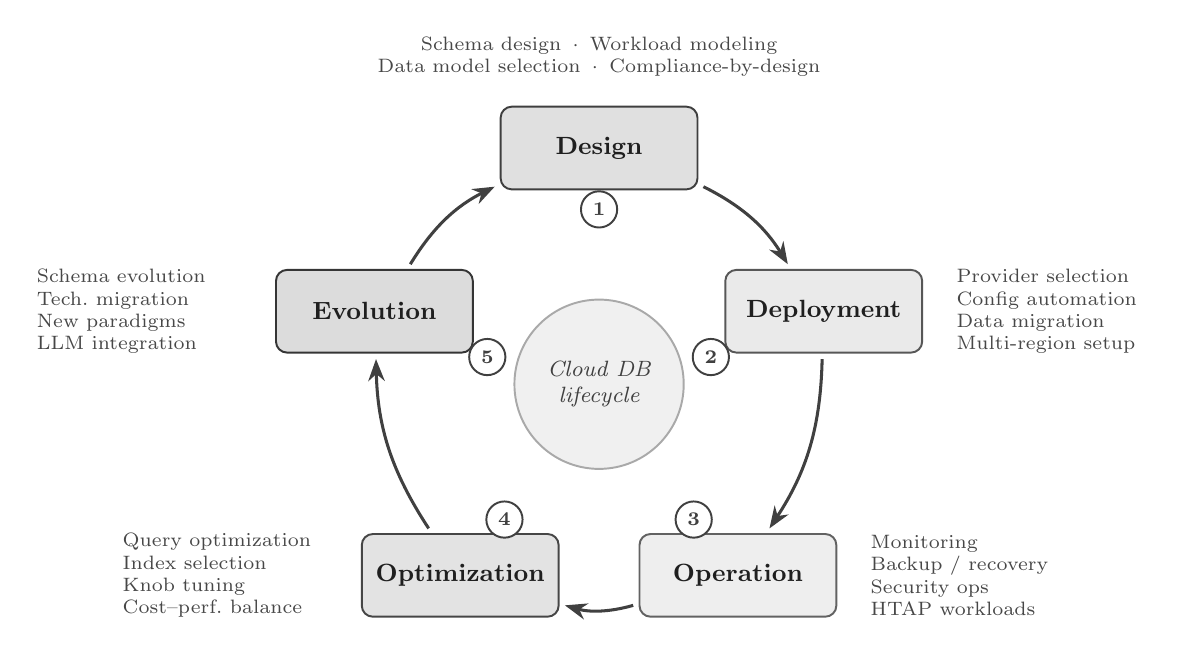
\begin{tikzpicture}[
    >=Stealth,
    phase/.style={
        draw=#1!55!black, fill=#1!22, line width=0.7pt, rounded corners=4pt,
        minimum width=2.5cm, minimum height=1.05cm, align=center,
        font=\small\bfseries, text=black!88},
    chal/.style={font=\scriptsize, align=left, text width=2.6cm, text=black!72},
    flow/.style={->, line width=1.1pt, draw=cdblue, shorten >=2pt, shorten <=2pt},
    seq/.style={circle, draw=cdblue, fill=white, line width=0.7pt, inner sep=0pt,
        minimum size=4.6mm, font=\scriptsize\bfseries, text=cdblue}
]
\def\R{3.0}

%% Phases on a regular pentagon, clockwise from the top
\node[phase=cblue,   label={[seq]270:1}] (design)   at (90:\R)   {Design};
\node[phase=corange, label={[seq]198:2}] (deploy)   at (18:\R)   {Deployment};
\node[phase=cgreen,  label={[seq]126:3}] (operate)  at (-54:\R)  {Operation};
\node[phase=cpurple, label={[seq]54:4}]  (optimize) at (-126:\R) {Optimization};
\node[phase=cred,    label={[seq]342:5}] (evolve)   at (162:\R)  {Evolution};

%% Central hub
\node[circle, draw=cdblue!45, fill=cdblue!8, line width=0.7pt, minimum size=2.15cm,
      align=center, font=\footnotesize\itshape, text=cdblue] (hub) at (0,0)
      {Cloud DB\\lifecycle};

%% Cyclic flow arrows hugging the ring (clockwise)
\draw[flow] (design)   to[bend left=16] (deploy);
\draw[flow] (deploy)   to[bend left=16] (operate);
\draw[flow] (operate)  to[bend left=16] (optimize);
\draw[flow] (optimize) to[bend left=16] (evolve);
\draw[flow] (evolve)   to[bend left=16] (design);

%% Key challenges, placed radially outward from each phase
\node[chal, above=2.5mm of design, text width=6cm, align=center]
   {Schema design \,$\cdot$\, Workload modeling\\ Data model selection \,$\cdot$\, Compliance-by-design};
\node[chal, right=3mm of deploy]
   {Provider selection\\ Config automation\\ Data migration\\ Multi-region setup};
\node[chal, right=3mm of operate]
   {Monitoring\\ Backup / recovery\\ Security ops\\ HTAP workloads};
\node[chal, left=3mm of optimize]
   {Query optimization\\ Index selection\\ Knob tuning\\ Cost--perf.\ balance};
\node[chal, left=3mm of evolve]
   {Schema evolution\\ Tech.\ migration\\ New paradigms\\ LLM integration};

\end{tikzpicture}
\caption{The cloud database lifecycle with key challenges mapped to each phase.}
\label{fig:lifecycle}
\end{figure}

\begin{table}[t]
\centering
\caption{Surveyed papers grouped by the lifecycle phase(s) they address (derived from the catalog in Table~\ref{tab:catalog}; a survey may span several phases, so the counts sum to more than~96). Representative examples are cited by S-ID; the complete per-phase assignment is part of the archived catalog data.}
\label{tab:lifecycle-phases}
\small
\begin{tabular}{p{1.9cm} >{\raggedright\arraybackslash}p{6.4cm} >{\raggedright\arraybackslash}p{3.2cm} c}
\toprule
\textbf{Phase} & \textbf{Representative challenges} & \textbf{Examples} & \textbf{\textit{n}} \\
\midrule
Design & Schema design, data-model selection, workload characterization, compliance-by-design & S6, S12, S53, S72, S91 & 60 \\
\addlinespace
Deployment & Provider selection \& lock-in, configuration automation, data ingestion/migration, multi-region setup & S4, S11, S22, S62, S93 & 23 \\
\addlinespace
Operation & Monitoring \& observability, backup/recovery, security operations, HTAP workload management & S1, S5, S16, S45, S80 & 47 \\
\addlinespace
Optimization & Learned query optimization, index/materialized-view selection, knob tuning, cost--performance balance & S2, S25, S37, S59, S88 & 74 \\
\addlinespace
Evolution & Schema evolution \& online DDL, technology migration, new-paradigm adoption, LLM integration & S4, S11, S39, S49, S65 & 7 \\
\bottomrule
\end{tabular}
\end{table}

\subsubsection{Design phase}
\label{subsubsec:design}

The design phase encompasses decisions made before a cloud database is deployed, including schema design, data model selection, workload characterization, and compliance architecture.

\textbf{Schema design for cloud-native environments.} Traditional schema design principles (normalization, ER modeling) must be adapted for cloud databases where denormalization may improve performance due to the cost of distributed joins~\cite{Li2024CloudNativeSurvey}. Document and wide-column stores require fundamentally different schema design approaches centered on access patterns rather than entity relationships~\cite{Davoudian2018NoSQL,Mouhibha2025NoSQLDW,Ferreira2023NoSQLMD,Mouhibha2026Clustering}.

\textbf{Workload characterization.} Accurate workload modeling is essential for selecting the right cloud database service, configuring resources, and estimating costs. Surveys on AI4DB~\cite{Zhou2022AI4DB} discuss workload forecasting using ML, but applying these techniques during the design phase---before production data exists---remains challenging.

\textbf{Data model selection.} Choosing between relational, document, graph, key-value, wide-column, vector, or multi-model databases requires understanding workload characteristics, query patterns, consistency requirements, and cost constraints. No systematic decision framework exists that accounts for all these dimensions~\cite{Lu2019MultiModel}.

\textbf{Compliance-by-design.} Incorporating regulatory requirements (GDPR, HIPAA, data sovereignty) into the initial database design rather than retrofitting compliance is increasingly recognized as essential~\cite{Politou2018GDPR}. This includes data residency constraints, encryption requirements, and audit trail design.

\subsubsection{Deployment phase}
\label{subsubsec:deployment}

The deployment phase covers provider selection, infrastructure configuration, data ingestion, and multi-region setup.

\textbf{Provider selection and vendor lock-in.} Choosing a cloud database provider involves evaluating technical capabilities, pricing, compliance certifications, geographic coverage, and ecosystem integration. Vendor lock-in---through proprietary features, APIs, and data formats---is consistently identified as a top concern across surveys~\cite{Opara2017LockIn,Li2024CloudNativeSurvey}.

\textbf{Configuration automation.} Infrastructure-as-Code (IaC) tools (Terraform, Pulumi, CloudFormation) enable automated database provisioning, but optimal configuration selection---instance types, storage tiers, replication settings, parameter tuning---often requires deep expertise that is difficult to automate~\cite{Zhang2022CDBTune}.

\textbf{Data ingestion and migration.} Initial data loading and ongoing ingestion from diverse sources (operational databases, streaming platforms, file systems) into cloud databases involves ETL/ELT pipeline design, schema mapping, and data quality assurance~\cite{Mathew2021CloudMigration}.

\textbf{Multi-region deployment.} Deploying databases across multiple geographic regions for latency, availability, and compliance reasons introduces challenges in data synchronization, conflict resolution, and region-aware routing~\cite{Corbett2013Spanner}.

\subsubsection{Operation phase}
\label{subsubsec:operation}

The operation phase covers the day-to-day management of running cloud database systems.

\textbf{Monitoring and observability.} Cloud databases generate vast amounts of telemetry data (metrics, logs, traces). Effective monitoring requires understanding normal behavior patterns, detecting anomalies, and correlating events across distributed components~\cite{Ma2021LearnedWorkload}. Work on self-driving databases~\cite{Pavlo2017SelfDriving} emphasizes the need for ML-driven anomaly detection and root cause analysis, and production experience with diagnosing intermittent slow queries at cloud scale shows how difficult root-cause attribution remains~\cite{Ma2020SlowQuery}.

\textbf{Backup, recovery, and disaster recovery.} While cloud providers automate basic backups (point-in-time recovery, snapshots), disaster recovery across regions, testing recovery procedures, and meeting stringent RPO/RTO targets remain operational challenges~\cite{Verbitski2017}.

\textbf{Security operations.} Ongoing security management includes access control auditing, encryption key rotation, vulnerability patching, network security configuration, and compliance monitoring. The dynamic nature of cloud environments (auto-scaling, serverless) complicates security posture management~\cite{Sanka2022CloudSecSurvey}.

\textbf{Real-time workload management (HTAP).} For HTAP systems~\cite{Haas2024HTAPSurvey}, operational challenges include managing resource contention between transactional and analytical workloads, maintaining freshness guarantees for analytical queries, and preventing analytical queries from degrading OLTP performance.

\subsubsection{Optimization phase}
\label{subsubsec:optimization}

The optimization phase encompasses techniques for improving performance and efficiency of running cloud databases.

\textbf{Learned query optimization.} ML-based query optimizers~\cite{Marcus2021Bao,Zhou2022AI4DB} that learn from workload history to generate better query plans represent a paradigm shift from traditional cost-based optimization. However, deploying learned optimizers in production requires addressing safety (avoiding catastrophic regressions), training efficiency, and adaptability to workload changes.

\textbf{Automated index and materialized view selection.} Cloud databases increasingly offer automated index recommendation (e.g., Azure SQL automatic tuning, Amazon Redshift automatic materialized views), but surveys~\cite{Zhou2022AI4DB} report that these systems are often conservative, covering only a fraction of possible optimizations.

\textbf{Knob tuning.} Database configuration parameters (buffer pool size, parallelism degree, checkpoint intervals, etc.) significantly impact performance. ML-based tuning systems~\cite{Zhang2022CDBTune,Tan2019iBTune} can explore the high-dimensional configuration space more effectively than manual tuning, but transferring tuning knowledge across different workloads and hardware remains an open problem.

\textbf{Cost--performance trade-off optimization.} In cloud environments, performance optimization cannot be divorced from cost. The optimal configuration minimizes cost subject to performance constraints (or maximizes performance subject to budget constraints), requiring multi-objective optimization~\cite{Leis2023CloudPricing}.

\subsubsection{Evolution phase}
\label{subsubsec:evolution}

The evolution phase addresses long-term changes in database systems, technologies, and requirements.

\textbf{Schema evolution and online DDL.} Changing database schemas in production without downtime (online DDL) is a critical capability for agile development. Cloud-native databases have improved online DDL support, but complex migrations (column type changes, table splits, data backfills) remain challenging~\cite{Li2024CloudNativeSurvey}.

\textbf{Technology migration.} Migrating from one database technology to another (e.g., from a relational database to a document store, or from a legacy system to a cloud-native database) is a major undertaking that surveys identify as poorly supported by existing tools~\cite{Mathew2021CloudMigration}.

\textbf{Adapting to new paradigms.} The emergence of vector databases for AI workloads~\cite{Pan2024VectorDB}, the lakehouse paradigm~\cite{Armbrust2021Lakehouse}, and serverless computing~\cite{Muller2020Serverless} requires existing systems to evolve or be replaced. Understanding when and how to adopt new paradigms is a strategic challenge.

\textbf{LLM integration.} The rapid rise of large language models (LLMs) is creating new requirements for cloud databases, from vector storage and retrieval for RAG pipelines to natural language interfaces for database querying and administration (discussed in detail in Section~\ref{sec:llm}).


%% ============================================================
%% SECTION 6: LLM CONVERGENCE
%% ============================================================
\section{Cloud Databases and Large Language Models---A Convergence Case Study}
\label{sec:llm}

The convergence of cloud databases and large language models (LLMs) represents one of the most dynamic and rapidly evolving areas in modern data management. This section examines this convergence as an illustrative case study, paralleling Saeed and Omlin's~\cite{Saeed2023XAI} treatment of XAI in medicine as a domain-specific application.

\subsection{LLM-augmented database interfaces}
\label{subsec:nl2sql}

Natural language interfaces to databases (NLIDB) have been a long-standing research goal~\cite{Affolter2019NLIDB}. The advent of LLMs has dramatically improved text-to-SQL accuracy, with systems like DIN-SQL~\cite{Pourreza2023DINSQL}, DAIL-SQL~\cite{Gao2023DAILSQL}, and MAC-SQL~\cite{Wang2024MACSQL} achieving over 85\% execution accuracy on the Spider benchmark~\cite{Yu2018Spider}.

\textbf{Current capabilities.} LLM-based text-to-SQL systems leverage schema-aware prompting, few-shot in-context learning, and chain-of-thought reasoning to translate natural language queries into SQL. Cloud vendors are integrating these capabilities: Amazon Q for databases, Azure AI integration with SQL, and Google Duet AI for BigQuery.

\textbf{Open challenges.}
\begin{itemize}
    \item Complex queries involving multiple joins, subqueries, and window functions remain error-prone.
    \item Schema understanding for large databases with hundreds of tables and complex relationships.
    \item Multi-turn conversational interfaces that maintain context across query refinements.
    \item Handling ambiguity, domain-specific terminology, and user intent clarification.
    \item Security risks from SQL injection through natural language prompts.
\end{itemize}

\subsection{Vector databases as LLM infrastructure}
\label{subsec:vectordb}

Vector databases have emerged as critical infrastructure for LLM applications, particularly retrieval-augmented generation (RAG) pipelines~\cite{Pan2024VectorDB}.

\textbf{Architecture and workloads.} RAG pipelines embed documents into high-dimensional vectors, store them in vector databases, and retrieve relevant context for LLM prompts based on semantic similarity. This creates unique workload patterns: bulk embedding ingestion, high-throughput approximate nearest neighbor (ANN) search, and hybrid queries combining vector similarity with metadata filtering.

\textbf{System landscape.} The vector database market has rapidly diversified, including purpose-built systems (Pinecone, Weaviate, Milvus, Qdrant, Chroma), vector extensions to existing databases (pgvector for PostgreSQL, Elasticsearch vector search), and cloud-native offerings (Amazon OpenSearch vector engine, Azure AI Search, Google Vertex AI Vector Search)~\cite{Pan2024VectorDB}.

\textbf{Open challenges.}
\begin{itemize}
    \item Scalability and freshness---keeping vector indexes up-to-date as source documents change.
    \item Multi-modal vector search combining text, image, and structured metadata.
    \item Quality metrics for retrieval that correlate with downstream LLM task performance.
    \item Cost optimization for storing and querying billions of high-dimensional vectors.
    \item Integration with existing cloud database ecosystems (transactions, access control, governance).
\end{itemize}

\subsection{LLMs for database administration}
\label{subsec:llmdba}

LLMs are increasingly applied to automate database administration tasks, including performance diagnosis, query optimization, and anomaly resolution.

\textbf{Systems and approaches.} D-Bot~\cite{Zhou2024DBot} uses LLMs for database diagnosis, performing root cause analysis of performance anomalies by querying system views and analyzing metrics. DB-GPT~\cite{Xue2024DBGPT} provides an LLM-powered framework for database interaction, supporting text-to-SQL, data analysis, and administration tasks. GPTuner~\cite{Lao2024GPTuner} leverages LLMs for database knob tuning, combining GPT-4 knowledge with Bayesian optimization.

\textbf{Open challenges.}
\begin{itemize}
    \item Reliability---LLMs can hallucinate incorrect diagnostic conclusions or generate harmful administration commands.
    \item Safety guardrails---preventing LLM-driven administration from executing destructive operations.
    \item Integrating LLM reasoning with structured database knowledge (system catalogs, performance models).
    \item Evaluation frameworks for LLM-based DBA tools that measure real-world effectiveness.
\end{itemize}

\subsection{Challenges and open problems at the convergence}
\label{subsec:llmchallenges}

The LLM--database convergence creates several overarching challenges:

\begin{enumerate}
    \item \textbf{Infrastructure co-design.} Jointly optimizing cloud database infrastructure for both traditional workloads and LLM-related workloads (embedding generation, vector search, context retrieval) requires new architectural thinking.

    \item \textbf{Data governance for AI.} Ensuring that LLM applications respect data access policies, privacy regulations, and audit requirements when retrieving context from cloud databases.

    \item \textbf{Evaluation and benchmarking.} Standardized benchmarks for vector database performance, text-to-SQL accuracy on real-world schemas, and LLM-based DBA effectiveness are needed.

    \item \textbf{Cost management.} LLM API calls combined with cloud database queries create complex cost structures that are difficult to predict and optimize.
\end{enumerate}

\subsection{What do we think? Open questions for cloud databases and LLMs}
\label{subsec:llmquestions}

Looking across the challenges catalogued in Section~\ref{sec:discussion}, the cloud-database--LLM convergence raises a set of questions that the surveyed literature has only begun to address. They are offered not as a checklist but as prompts for future work in this domain---and, by analogy, for other data-intensive domains:
\begin{itemize}
  \item How should a cloud database co-schedule traditional query workloads and LLM-driven workloads (embedding generation, vector search, context retrieval) on shared, elastic infrastructure without one starving the other?
  \item When an LLM retrieves context from governed cloud data, how can access policies, privacy regulations, and audit obligations be enforced \emph{through} the retrieval path rather than around it?
  \item What would a faithful benchmark for this convergence measure---vector-search quality, text-to-SQL accuracy on real enterprise schemas, or the end-to-end utility of an LLM-assisted DBA---and who maintains its ground truth?
  \item Can the reliability of LLM-based administration be bounded well enough to let it act on production systems, and what guardrails make graceful degradation the default when the model is wrong?
  \item How should the combined cost of LLM inference and cloud-database execution be modeled and optimized as a single objective, given that today they are billed and tuned independently?
  \item What role can knowledge graphs and ontologies play in grounding LLM reasoning in the actual schema, constraints, and semantics of a cloud database---turning a plausible answer into a correct one?
\end{itemize}

These questions show how the cross-cutting and lifecycle challenges of Section~\ref{sec:discussion} resurface, sharpened, when cloud databases meet LLMs; the same analysis could be re-instantiated for other domains such as scientific data management or real-time analytics.


%% ============================================================
%% SECTION 7: CONCLUSIONS
%% ============================================================
\section{Conclusions}
\label{sec:conclusion}

This paper has presented the first systematic meta-survey of cloud database research, synthesizing findings from 96 content-verified survey papers identified through a reproducible, scripted search covering January 1999 to July 2026. Applying the Kitchenham--Charters protocol with PRISMA~2020 reporting, the scattered landscape of cloud database challenges has been consolidated into a structured, dual-theme taxonomy.

For the first theme, eighteen cross-cutting challenges are identified and synthesized: (1)~scalability and elasticity; (2)~consistency and the CAP/PACELC trade-offs; (3)~performance optimization and benchmarking; (4)~security and privacy; (5)~cost modeling and optimization; (6)~multi-tenancy and resource isolation; (7)~data-model diversity and multi-model integration; (8)~heterogeneous query processing; (9)~storage disaggregation and the log-as-database pattern; (10)~distributed transaction processing; (11)~fault tolerance, recovery, and high availability; (12)~data migration and cross-cloud portability; (13)~the edge--cloud data continuum; (14)~AI--database convergence; (15)~serverless and autonomous operation; (16)~data governance, provenance, and lineage; (17)~sustainability and energy efficiency; and (18)~standardization and interoperability. Across these, \emph{scalability}, \emph{consistency}, \emph{security}, \emph{cost}, and \emph{AI--database convergence} recur in the majority of the surveyed domains (Table~\ref{tab:challenge-year}), indicating where progress would benefit the field most broadly.

For the second theme, the challenges are mapped to the five phases of the cloud database lifecycle---design, deployment, operation, optimization, and evolution. Design and optimization are the most thoroughly surveyed phases, whereas evolution (schema change, technology migration, and new-paradigm adoption) is the least mature and most under-served (Table~\ref{tab:lifecycle-phases}), making it a particularly promising target for future work.

Two observations cut across both themes. The convergence of cloud databases with large language models is moving rapidly from research to practice through vector databases, text-to-SQL, and LLM-based administration, yet reliability, governance, and evaluation remain unresolved (Section~\ref{sec:llm}). And from a knowledge-engineering standpoint, cloud databases offer rich openings for DKE techniques---knowledge graphs for metadata and lineage, ontology-mediated integration and query answering, and formal models for consistency, cost, and schema evolution.

Accordingly, this meta-survey is intended to serve three purposes: (1)~as a comprehensive reference for researchers entering the cloud database space, providing a structured map of the territory and its open problems; (2)~as a strategic guide for practitioners navigating technology selection, deployment, and evolution; and (3)~as a bridge between the cloud database and the data-and-knowledge-engineering communities.

\textbf{Limitations.} Three limitations qualify these conclusions. First, the corpus is deliberately restricted to surveys that could be content-verified against a resolvable DOI or arXiv identifier, trading breadth for confirmability, so some relevant but harder-to-verify or paywalled surveys may be absent. Second, study selection, quality assessment, and data extraction were performed by a single reviewer (Section~\ref{subsec:threats}). Third, as a survey of surveys, the findings inherit the currency limitations of the primary surveys, so the fastest-moving topics---most notably LLM--database convergence---may be under-represented relative to their present activity.

\subsection*{Future work}

Based on the analysis of 96 surveys and the challenges discussed in Sections~\ref{sec:discussion} and~\ref{sec:llm}, several priority research directions emerge:
\begin{itemize}
  \item \textbf{Foundational systems.} Cloud-native benchmarks that capture elasticity, multi-tenancy, and pricing; the transition of learned optimizers, learned indexes, and ML-based tuning from prototypes to production-ready, safely-degrading components; and a maturing vector-database ecosystem with standardized APIs and retrieval-quality metrics.
  \item \textbf{Architecture and query processing.} Cross-cloud middleware and portable open formats that reduce vendor lock-in; and federated query processing with consistent transactions across heterogeneous engines and the edge--fog--cloud continuum.
  \item \textbf{Intelligence and autonomy.} Autonomous databases whose learned decisions are explainable and grounded in database knowledge; and intent-driven natural-language interfaces that let users express goals directly while preserving correctness and access control.
  \item \textbf{Governance and sustainability.} Privacy-preserving analytics and end-to-end lineage that scale to regulatory needs; and energy- and carbon-aware database operation that converges the relational, graph, document, vector, and streaming models toward unified, sustainable platforms.
\end{itemize}

\section*{Declaration of competing interest}
The authors declare that they have no known competing financial interests or personal relationships that could have appeared to influence the work reported in this paper.

\section*{Data availability}
This study analyzes previously published survey papers, all of which are cited in the manuscript. The complete identification and selection pipeline is archived with the manuscript sources: the search scripts (\texttt{search/search\_surveys.py} and companions), the per-query search log (\texttt{search\_log.json}), the deduplicated candidate pool (\texttt{candidates.csv}), the per-record screening-decision log covering every stage of the PRISMA flow (\texttt{screening\_decisions.csv}), the quality-assessment scores (\texttt{qa\_scores.csv}), and the frozen machine-readable catalog (\texttt{catalog.csv}) from which every figure and table in Section~\ref{subsec:results} is generated. This permits verbatim re-execution of the search and independent audit of every inclusion decision.

%% ============================================================
%% APPENDIX
%% ============================================================
\appendix
\section{Complete List of Surveyed Papers with Classification}
\label{app:catalog}

Table~\ref{tab:catalog} presents the complete catalog of the 96 surveyed papers, classified by primary topic, year, venue, quality-assessment score, and lifecycle phases covered.

\begin{landscape}
\begin{longtable}{c p{4.2cm} c p{2.1cm} p{2.4cm} c p{3.2cm}}
\caption{Master catalog of surveyed papers (S1--S96), ordered chronologically. QA = quality-assessment score (out of 8; inclusion threshold $\geq$6).} \label{tab:catalog} \\
\toprule
\textbf{ID} & \textbf{Title (Abbreviated)} & \textbf{Year} & \textbf{Primary Topic} & \textbf{Venue} & \textbf{QA} & \textbf{Lifecycle Phases} \\
\midrule
\endfirsthead
\toprule
\textbf{ID} & \textbf{Title (Abbreviated)} & \textbf{Year} & \textbf{Primary Topic} & \textbf{Venue} & \textbf{QA} & \textbf{Lifecycle Phases} \\
\midrule
\endhead
\midrule
\multicolumn{7}{r}{\textit{Continued on next page}} \\
\endfoot
\bottomrule
\endlastfoot
S1 & Database as a Service: Challenges and solutions for privacy and\ldots{}~\cite{Ferrari2009DBaaSSec} & 2009 & Security/Privacy & IEEE APSCC & 6 & Operate \\
\addlinespace
S2 & An in-depth comparison of subgraph isomorphism algorithms in gr\ldots{}~\cite{Lee2012GraphDB} & 2012 & Graph Databases & PVLDB & 6.5 & Optimize \\
\addlinespace
S3 & A Survey of Cloud Database Systems~\cite{Deka2014CloudDBSurvey} & 2014 & NoSQL/NewSQL & IEEE IT Professional & 6 & Design, Operate, Optimize \\
\addlinespace
S4 & A Systematic Review of Cloud Computing, Big Data and Databases \ldots{}~\cite{Litchfield2014DBaaS} & 2014 & DBaaS & AMCIS & 8 & Design, Deploy, Operate, Optimize, Evolve \\
\addlinespace
S5 & Confidential database-as-a-service approaches: taxonomy and sur\ldots{}~\cite{Kohler2015Sec} & 2015 & Security/Privacy & J. Cloud Comput. & 7.5 & Design, Operate, Optimize \\
\addlinespace
S6 & Choosing the right NoSQL database for the job: a quality attrib\ldots{}~\cite{Lourenco2015NoSQL} & 2015 & NoSQL/NewSQL & J. Big Data & 7.5 & Design, Operate, Optimize \\
\addlinespace
S7 & Transaction Management Techniques and Practices in Current Clou\ldots{}~\cite{Waqas2015DistDB} & 2015 & Distributed DBs & IJDMS & 7 & Design, Operate, Optimize \\
\addlinespace
S8 & Database-as-a-Service for Big Data: An Overview~\cite{Abourezq2016DBaaS} & 2016 & DBaaS & IJACSA & 7 & Design, Deploy, Operate, Optimize \\
\addlinespace
S9 & Query Optimization Techniques in Graph Databases~\cite{Ammar2016GraphDB} & 2016 & Graph Databases & IJDMS & 7 & Optimize \\
\addlinespace
S10 & Some problems on graph databases~\cite{Guralnik2016GraphDB} & 2016 & Graph Databases & Proc. ISP RAS & 7 & Optimize \\
\addlinespace
S11 & Cloud Migration Process: A Survey~\cite{Mathew2021CloudMigration} & 2016 & Cloud DB Migration & J. Syst. Softw. & 7.5 & Deploy, Evolve \\
\addlinespace
S12 & Foundations of Query Languages for Graph DBs~\cite{Angles2020GraphDB} & 2017 & Graph Databases & ACM Comp. Surv. & 8 & Design, Optimize \\
\addlinespace
S13 & Open Source Time Series Databases: A Survey~\cite{Bader2017TSDB} & 2017 & Time-Series DBs & BTW & 6 & Design, Operate \\
\addlinespace
S14 & A Survey on Graph Queries Processing: Techniques and Methods~\cite{Dinari2017GraphDB} & 2017 & Graph Databases & IJCNIS & 6.5 & Optimize \\
\addlinespace
S15 & Survey on Security Mechanisms In NoSQL Databases~\cite{Dindoliwala2017Sec} & 2017 & Security/Privacy & IJARCS & 6 & Operate \\
\addlinespace
S16 & Enforcing Privacy in Cloud Databases~\cite{Moghadam2017Sec} & 2017 & Security/Privacy & arXiv & 6.5 & Operate, Optimize \\
\addlinespace
S17 & Big data storage technologies: a survey~\cite{Siddiqa2017NoSQL} & 2017 & NoSQL/NewSQL & Front. Inf. Technol. Electron. Eng. & 7.5 & Design, Operate \\
\addlinespace
S18 & Evolutionary Algorithms for Query Op-timization in Distributed \ldots{}~\cite{Ali2018AI4DB} & 2018 & AI4DB/Learned Opt. & ADCAIJ & 6 & Optimize \\
\addlinespace
S19 & A Survey on NoSQL Stores~\cite{Davoudian2018NoSQL} & 2018 & NoSQL/NewSQL & ACM Comp. Surv. & 8 & Design, Deploy \\
\addlinespace
S20 & Saving Large Semantic Data in Cloud: A Survey of the Main DBaaS\ldots{}~\cite{Iancu2018DBaaS} & 2018 & DBaaS & Informatica Economica & 6 & Design, Deploy \\
\addlinespace
S21 & A Survey on Graph Database Management Techniques for Huge Unstr\ldots{}~\cite{Patil2018GraphDB} & 2018 & Graph Databases & IJECE & 7 & Design, Optimize \\
\addlinespace
S22 & DBaaS Multitenancy, Auto-tuning and SLA Maintenance in Cloud En\ldots{}~\cite{Segalin2018DBaaS} & 2018 & DBaaS & iSys & 7 & Deploy, Operate, Optimize \\
\addlinespace
S23 & Recent NL Interfaces for Databases: A Comparative Survey~\cite{Affolter2019NLIDB} & 2019 & NL/LLM-Database & VLDB Journal & 7.5 & Optimize \\
\addlinespace
S24 & Consistency models in distributed systems: A survey on definiti\ldots{}~\cite{Aldin2019DistDB} & 2019 & Distributed DBs & arXiv & 6 & Operate, Optimize \\
\addlinespace
S25 & Database Query Optimization using Genetic Algorithms: A Systema\ldots{}~\cite{Chande2019AI4DB} & 2019 & AI4DB/Learned Opt. & IJATCSE & 7.5 & Optimize \\
\addlinespace
S26 & Frameworks for Querying Databases Using Natural Language: A Lit\ldots{}~\cite{Dar2019NLIDB} & 2019 & NL/LLM-Database & arXiv & 6.5 & Optimize \\
\addlinespace
S27 & Architecture, Security \& Performance of DBaaS~\cite{Khan2019DaaSAnalytic} & 2019 & Security/Privacy & Trans. Emerg. Telecom. Tech. & 6.5 & Design, Operate \\
\addlinespace
S28 & A comparative analysis of adaptive consistency approaches in cl\ldots{}~\cite{Khelaifa2019DistDB} & 2019 & Distributed DBs & J. Parallel Distrib. Comput. & 7.5 & Operate, Optimize \\
\addlinespace
S29 & Multi-Model Databases: A New Journey~\cite{Lu2019MultiModel} & 2019 & Multi-Model DBs & ACM Comp. Surv. & 8 & Design, Deploy \\
\addlinespace
S30 & LSM-based storage techniques: a survey~\cite{Luo2019NoSQL} & 2019 & NoSQL/NewSQL & VLDB J. & 7.5 & Design, Optimize \\
\addlinespace
S31 & The Query Translation Landscape: a Survey~\cite{Mami2019MultiModel} & 2019 & Multi-Model DBs & arXiv & 6.5 & Optimize \\
\addlinespace
S32 & Blockchains vs. Distributed Databases: Dichotomy and Fusion~\cite{Ruan2019DistDB} & 2019 & Distributed DBs & arXiv & 6 & Design, Operate, Optimize \\
\addlinespace
S33 & NoSQL Databases: Yearning for Disambiguation~\cite{Asaad2020NoSQL} & 2020 & NoSQL/NewSQL & arXiv & 6 & Design, Operate \\
\addlinespace
S34 & Benchmarking Graph Data Management and Processing Systems: A Su\ldots{}~\cite{Dayarathna2020Bench} & 2020 & Benchmarking & arXiv & 6.5 & Optimize \\
\addlinespace
S35 & SQL, NewSQL, and NoSQL Databases: A Comparative Survey~\cite{Khasawneh2020SQLNewSQL} & 2020 & NoSQL/NewSQL & IEEE ICICS & 6 & Design, Deploy \\
\addlinespace
S36 & Real-time analytics, hybrid transactional/analytical processing\ldots{}~\cite{Kuznetsov2020HTAP} & 2020 & HTAP Systems & Proc. ISP RAS & 6.5 & Design, Optimize \\
\addlinespace
S37 & Benchmarking learned indexes~\cite{Marcus2020AI4DB} & 2020 & AI4DB/Learned Opt. & PVLDB & 7.5 & Optimize \\
\addlinespace
S38 & Querying in the Age of Graph Databases and Knowledge Graphs~\cite{Arenas2021GraphDB} & 2021 & Graph Databases & ACM SIGMOD Record & 6.5 & Design, Optimize \\
\addlinespace
S39 & Big Data Storage Tools Using NoSQL Databases and Their Applicat\ldots{}~\cite{Faridoon2021NoSQL} & 2021 & NoSQL/NewSQL & Computing and Informatics & 8 & Design, Operate, Optimize, Evolve \\
\addlinespace
S40 & Evaluation of Distributed Databases in Hybrid Clouds and Edge C\ldots{}~\cite{Mansouri2021EdgeFog} & 2021 & Edge/Fog DBs & arXiv (Cornell University) & 6.5 & Design, Deploy, Optimize \\
\addlinespace
S41 & Comparison and evaluation of state-of-the-art LSM merge policies~\cite{Mao2021NoSQL} & 2021 & NoSQL/NewSQL & VLDB J. & 7.5 & Optimize \\
\addlinespace
S42 & Cloud Computing Security: Threats \& Mitigation--An SLR~\cite{Sanka2022CloudSecSurvey} & 2021 & Security/Privacy & IEEE Access & 7 & Operate \\
\addlinespace
S43 & Constructing and analyzing the LSM compaction design space~\cite{Sarkar2021NoSQL} & 2021 & NoSQL/NewSQL & PVLDB & 7.5 & Design, Optimize \\
\addlinespace
S44 & The Forgotten Document-Oriented Database Management Systems: An\ldots{}~\cite{Truica2021NoSQL} & 2021 & NoSQL/NewSQL & Big Data Research & 7.5 & Design, Optimize \\
\addlinespace
S45 & Integrity Authentication for SQL Query Evaluation on Outsourced\ldots{}~\cite{Zhang2021Sec} & 2021 & Security/Privacy & IEEE TKDE & 7.5 & Operate \\
\addlinespace
S46 & Towards Polyglot Data Stores -- Overview and Open Research Ques\ldots{}~\cite{Glake2022MultiModel} & 2022 & Multi-Model DBs & arXiv & 6.5 & Design, Optimize \\
\addlinespace
S47 & From Data Warehouse to Lakehouse: A Comparative Review~\cite{Harby2022Lakehouse} & 2022 & Data Lakehouse & IEEE BigData & 6.5 & Design, Deploy \\
\addlinespace
S48 & A Survey of Comparison Different Cloud Database Performance: SQ\ldots{}~\cite{Shareef2022NoSQL} & 2022 & NoSQL/NewSQL & Passer J. & 7 & Design, Deploy, Operate, Optimize \\
\addlinespace
S49 & Database Meets AI: A Survey~\cite{Zhou2022AI4DB} & 2022 & AI4DB/Learned Opt. & IEEE TKDE & 8 & Optimize, Evolve \\
\addlinespace
S50 & Consistency issue and related trade-offs in distributed replica\ldots{}~\cite{Ahmed2023DistDB} & 2023 & Distributed DBs & Radioelectron. Comput. Syst. & 7 & Design, Operate, Optimize \\
\addlinespace
S51 & Demystifying Graph Databases: Analysis and Taxonomy of Data Org\ldots{}~\cite{Besta2023GraphDB} & 2023 & Graph Databases & ACM Comput. Surv. & 8 & Design, Operate, Optimize \\
\addlinespace
S52 & Multidimensional Modelling in NoSQL Database : A Systematic Rev\ldots{}~\cite{Ferreira2023NoSQLMD} & 2023 & NoSQL/NewSQL & CISTI & 7.5 & Design \\
\addlinespace
S53 & Multi-model query languages: taming the variety of big data~\cite{Guo2023MultiModel} & 2023 & Multi-Model DBs & Distrib. Parallel Databases & 7.5 & Design, Optimize \\
\addlinespace
S54 & SQL and NoSQL Database Software Architecture Performance Analys\ldots{}~\cite{Khan2023NoSQL} & 2023 & NoSQL/NewSQL & Big Data Cogn. Comput. & 8 & Design, Deploy, Optimize \\
\addlinespace
S55 & A Survey on Property-Preserving Database Encryption Techniques \ldots{}~\cite{Koppenwallner2023Sec} & 2023 & Security/Privacy & arXiv & 6.5 & Design, Operate, Optimize \\
\addlinespace
S56 & A Comprehensive Survey on Vector Database: Storage and Retrieva\ldots{}~\cite{Ma2023VectorDB} & 2023 & Vector Databases & arXiv & 7.0 & Design, Optimize, Operate \\
\addlinespace
S57 & The World of Graph Databases from An Industry Perspective~\cite{Tian2023GraphDB} & 2023 & Graph Databases & ACM SIGMOD Rec. & 7.5 & Design, Operate, Optimize \\
\addlinespace
S58 & An Overview on Cloud Distributed Databases for Business Environ\ldots{}~\cite{Vikiru2023DBaaS} & 2023 & DBaaS & arXiv & 6 & Design, Deploy, Operate, Optimize \\
\addlinespace
S59 & Learned Index: A Comprehensive Experimental Evaluation~\cite{Woltmann2023DNNIndex} & 2023 & AI4DB/Learned Opt. & PVLDB & 7 & Optimize \\
\addlinespace
S60 & Understanding Graph Databases: A Comprehensive Tutorial and Sur\ldots{}~\cite{Anuyah2024GraphDB} & 2024 & Graph Databases & arXiv & 6 & Design, Optimize \\
\addlinespace
S61 & Energy Consumption and Performance Evaluation of Multi-Model No\ldots{}~\cite{Falcao2024Bench} & 2024 & Benchmarking & R. Inform. Teor. Apl. & 7 & Design, Optimize \\
\addlinespace
S62 & Retrieval-Augmented Generation for LLMs: A Survey~\cite{Gao2024RAGSurvey} & 2024 & NL/LLM-Database & arXiv & 7 & Deploy, Operate \\
\addlinespace
S63 & Databases in Edge and Fog Environments: A Survey~\cite{Gomes2024EdgeFog} & 2024 & Edge/Fog DBs & ACM Comp. Surv. & 7.5 & Design, Deploy, Operate \\
\addlinespace
S64 & HTAP Databases: A Survey~\cite{Haas2024HTAPSurvey} & 2024 & HTAP Systems & arXiv & 6.5 & Design, Operate, Optimize \\
\addlinespace
S65 & The evolution of data storage architectures: examining the secu\ldots{}~\cite{Janssen2024Lakehouse} & 2024 & Data Lakehouse & J. Data Inf. Manag. & 7.5 & Design, Operate, Evolve \\
\addlinespace
S66 & Cloud-Native Databases: A Survey~\cite{Li2024CloudNativeSurvey} & 2024 & Cloud-Native Arch. & IEEE TKDE & 8 & Design, Deploy, Operate, Optimize \\
\addlinespace
S67 & A survey of LSM-Tree based Indexes, Data Systems and KV-stores~\cite{Mishra2024NoSQL} & 2024 & NoSQL/NewSQL & IEEE SCEECS & 7.5 & Design, Optimize \\
\addlinespace
S68 & A Systematic Review of Automated Classification for Simple and \ldots{}~\cite{Nurhadi2024AI4DB} & 2024 & AI4DB/Learned Opt. & Comput. Syst. Sci. Eng. & 7.5 & Optimize, Operate \\
\addlinespace
S69 & Survey of Vector Database Management Systems~\cite{Pan2024VectorDB} & 2024 & Vector Databases & VLDB Journal & 7.5 & Design, Deploy, Optimize \\
\addlinespace
S70 & Data Lakehouse for Time Series Data: An SLR~\cite{Pohl2024LakehouseTS} & 2024 & Data Lakehouse & IEEE BigData & 6.5 & Design, Operate \\
\addlinespace
S71 & Data Modeling for Connected Data -- A systematic literature rev\ldots{}~\cite{Santos2024GraphDB} & 2024 & Graph Databases & arXiv & 7 & Design, Evolve \\
\addlinespace
S72 & Database Security Issues and Challenges in Cloud Computing~\cite{Satish2024Sec} & 2024 & Security/Privacy & IJRITCC & 6.5 & Design, Operate \\
\addlinespace
S73 & Sharding Distributed Databases: A Critical Review~\cite{Solat2024DistDB} & 2024 & Distributed DBs & arXiv & 6 & Design, Operate, Optimize \\
\addlinespace
S74 & A survey on hybrid transactional and analytical processing~\cite{Song2024HTAP} & 2024 & HTAP Systems & VLDB J. & 7.5 & Design, Optimize \\
\addlinespace
S75 & DBMS Performance Comparisons: An SLR~\cite{Taipalus2024DBMSPerf} & 2024 & Benchmarking & J. Syst. Softw. & 7.5 & Optimize \\
\addlinespace
S76 & Vector database management systems: Fundamental concepts, use-c\ldots{}~\cite{Taipalus2024VectorDB} & 2024 & Vector Databases & Cogn. Syst. Res. & 7.5 & Design, Operate, Optimize \\
\addlinespace
S77 & Cassandra vs. MongoDB: A Systematic Review~\cite{Tu2024CassandraMongo} & 2024 & NoSQL/NewSQL & IEEE BDAI & 6 & Design, Optimize \\
\addlinespace
S78 & Automatic Configuration Tuning on Cloud Database: A Survey~\cite{Zhang2024AI4DB} & 2024 & AI4DB/Learned Opt. & arXiv & 6.5 & Optimize, Operate \\
\addlinespace
S79 & A Survey of Learned Indexes for the Multi-dimensional Space~\cite{AbdullahAlMamun2025AI4DB} & 2025 & AI4DB/Learned Opt. & ACM Comput. Surv. & 7.5 & Design, Optimize \\
\addlinespace
S80 & AI-Powered Database Management: Predictive Analytics for Perfor\ldots{}~\cite{Ali2025AI4DB} & 2025 & AI4DB/Learned Opt. & Eng. Technol. J. & 7 & Optimize, Operate \\
\addlinespace
S81 & Survey: On the Landscape of Graph Databases~\cite{Coimbra2025GraphDB2} & 2025 & Graph Databases & arXiv & 7 & Design, Deploy, Operate, Optimize \\
\addlinespace
S82 & Evaluating Performance and User Perceptions of Multi-Cloud Data\ldots{}~\cite{Daundasekara2025MultiCloud} & 2025 & DBaaS & IEEE ICAC & 6.5 & Deploy, Operate, Optimize \\
\addlinespace
S83 & A Survey on Distributed Database Systems in the Era of Big Data~\cite{Hasan2025DistDB} & 2025 & Distributed DBs & Eng. Technol. J. & 6 & Design, Operate, Optimize \\
\addlinespace
S84 & When Large Language Models Meet Vector Databases: A Survey~\cite{Jing2025NLIDB} & 2025 & NL/LLM-Database & arXiv & 7 & Design, Optimize \\
\addlinespace
S85 & NoSQL Databases: A Survey~\cite{Kaur2021NoSQLReview} & 2025 & NoSQL/NewSQL & ARIMA & 7.5 & Design, Deploy \\
\addlinespace
S86 & Graph Neural Networks for Databases: A Survey~\cite{Li2025AI4DB} & 2025 & AI4DB/Learned Opt. & arXiv & 6.5 & Optimize \\
\addlinespace
S87 & Evaluating Learned Indexes in LSM-tree Systems: Benchmarks,Insi\ldots{}~\cite{Liu2025AI4DB} & 2025 & AI4DB/Learned Opt. & arXiv & 6.5 & Optimize \\
\addlinespace
S88 & How good are multi-dimensional learned indexes? An experimental\ldots{}~\cite{Liu2025Bench} & 2025 & Benchmarking & VLDB J. & 7.5 & Optimize \\
\addlinespace
S89 & Data Integrity and Consistency Challenges in Distributed Databa\ldots{}~\cite{Mahmoud2025DistDB} & 2025 & Distributed DBs & Eng. Technol. J. & 6.5 & Design, Operate, Optimize \\
\addlinespace
S90 & Survey on Cloud Database Security: Cryptographic Techniques, In\ldots{}~\cite{Mahule2025Sec} & 2025 & Security/Privacy & EPJ Web Conf. & 7.5 & Operate, Optimize \\
\addlinespace
S91 & NoSQL Data Warehouse Optimizing Models~\cite{Mouhibha2025NoSQLDW} & 2025 & NoSQL/NewSQL & Big Data Research & 6 & Design, Optimize \\
\addlinespace
S92 & Learning database optimization techniques: the state-of-the-art\ldots{}~\cite{Qiao2025AI4DB} & 2025 & AI4DB/Learned Opt. & Front. Comput. Sci. & 7.5 & Optimize \\
\addlinespace
S93 & Evaluating the Performance of NoSQL Databases for Big Data in C\ldots{}~\cite{Topcu2025NoSQL} & 2025 & NoSQL/NewSQL & HighTech Innov. J. & 7.5 & Deploy, Optimize \\
\addlinespace
S94 & Toward Understanding Bugs in Vector Database Management Systems~\cite{Xie2025VectorDB} & 2025 & Vector Databases & arXiv & 7 & Deploy, Operate, Optimize \\
\addlinespace
S95 & Comparative Analysis of SQL and NoSQL Databases: Data Models, U\ldots{}~\cite{Ying2025NoSQL} & 2025 & NoSQL/NewSQL & Info. Res. Commun. & 7 & Design, Operate, Optimize \\
\addlinespace
S96 & A Survey of Emerging Trends and Algorithmic Solutions inCloud-N\ldots{}~\cite{Allam2026CloudNative} & 2026 & Cloud-Native Arch. & JSAA & 7.5 & Design, Deploy, Operate, Optimize, Evolve \\
\end{longtable}
\end{landscape}


%% ============================================================
%% BIBLIOGRAPHY
%% ============================================================
\bibliographystyle{elsarticle-num}
\bibliography{cloud-db-metasurvey}

\end{document}
